\documentclass[a4paper, twocolumn]{article}

% Included packages ---------------------------------------------------------- %
\usepackage{lipsum}                          % Generate random, blind, filler-text.
\usepackage[utf8]{inputenc}                  % utf-8 encoding, æ, ø , å, etc.
\usepackage{a4wide}                          % Adjust margins to better fit A4 format.
\usepackage{array}                           % Matrices.
\usepackage{dsfont}                          % Math symbols.
\usepackage{amsmath}                         % Math symbols, and enhanced matrices.
\usepackage{amsfonts}                        % Math fonts.
\usepackage{amssymb}                         % Additional symbols.
\usepackage{mathrsfs}                        % Most additional symbols.
\usepackage[pdftex]{graphicx}                % Improved inclusion of .pdf-graphics files.
\usepackage{sidecap}                         % Floats with captions to the right/left.
\usepackage{enumerate}                       % Change counters (arabic, roman, etc.).
\usepackage{floatrow}                        % Multi-figure floats.
\usepackage{subfig}                          % Multi-figure floats.
\usepackage{bm}                              % Bolded text in math mode.
\usepackage[framemethod=default]{mdframed}   % Make boxes.
\usepackage{listings}                        % For including source code.
\usepackage{mathtools}                       % Underbrackets, overbrackets.
\usepackage[dvipsnames]{xcolor}              % Colors.
\usepackage{capt-of}                         % Caption things which are not floats.
\usepackage{algorithm2e}                     % Algorithm non-float which we can caption by \captionof{algocf}{<caption>}.
\usepackage{fontawesome}                     % Github icon, etc. \faGithub
\usepackage{sidecap}                         % Floats with captions on the side.
\usepackage{tabularx}                        % Tables and stuff.
\usepackage{tabulary}                        % Tables and stuff.
\usepackage[sf,sl,outermarks]{titlesec}      % Change fonts in section{}, subsection{}, etc.
\usepackage[subfigure]{tocloft}              % Change spacing between numbers and titles in TOC.
\usepackage{pgfplots}                        % Making Tikz plots.
\usepackage{booktabs}                        % \toprule, \midrule, etc. for tables.
\usepackage{siunitx}                         % Allows S table column, aligning on decimal point.
\usepackage{chngcntr}                        % Change counter behaviour, supress increment of sub counters.
\usepackage{tikz}                            % Draw complicated pictures in a super hard way.
\usepackage{cuted}                           % Place long equations in @twocolumn over entire page.
\usepackage[version=4]{mhchem}               % Chemical reaction equations using \ce{...}.
\usepackage[%                                % Adds functionality to captions.
  tableposition = top,
  labelsep      = period,
  justification = raggedright,
  format        = hang,
  ]{caption}                                 
\usepackage[%                                % Interactive references and links, colored.
  colorlinks  = true,
  linkcolor   = black,
  urlcolor    = blue,
  citecolor   = black,
  linktocpage = true,
  ]{hyperref}            
\usepackage[%                                % References, in super-script form.
  autocite    = superscript,
  backend     = biber,
  sortcites   = true,
  style       = numeric-comp,
  sorting     = none,
  url         = false,
  ]{biblatex}
\usepackage[autostyle, english = american]{csquotes} % Assure quotation marks are inserted correctly aligned left/right.
\MakeOuterQuote{"}

% Package settings ----------------------------------------------------------- %
\renewcommand{\thesection}{\Roman{section}}         % I, II, III, IV, etc. section numbering
\renewcommand{\thesubsection}{\Alph{subsection}}    % A, B, C, etc. subsection numbering
\renewcommand{\thesubsubsection}{}                  % Remove subsubsection numbering.
\floatsetup[table]{capposition=top}                 % Place table captions above the table.
\captionsetup[subfigure]{labelformat=empty}         % Remove the (a), (b), etc. tags from subfigures.
\advance\cftsecnumwidth 1.0em\relax                 % Set the spacing between section headings and titles in TOC with tocloft.
\advance\cftsubsecindent 1.0em\relax                % Set the spacing between subsection headings and titles in TOC with tocloft.
\advance\cftsubsecnumwidth 1.0em\relax              % Set the spacing between subsubsection headings and titles in TOC with tocloft.
\newcommand{\listingsfont}{\ttfamily}
\newcommand{\inlinepy}[1]{\lstinline[language={python}]{#1}}
\newcommand{\inlinecc}[1]{\lstinline[language={c++}]{#1}}
\counterwithout*{subsection}{section}               % Dont reset the subsection counter on new \section{} calls.
\renewcommand{\figurename}{FIG.}                    % Captions of figures read FIG.
\renewcommand{\tablename}{TABLE}                    % Captions of tables read TABLE 
\renewcommand{\thetable}{\Roman{table}}             % Number tables with roman numerals.
\usetikzlibrary{matrix}                             % Some tikz picture library things.
\usetikzlibrary{arrows.meta, calc, chains, positioning}
\definecolor{listingsbackgroundcolor}{rgb}{0.975,0.975,0.975}
\colorlet{shadecolor}{listingsbackgroundcolor}



% Section headings settings -------------------------------------------------- %
\titleformat{\section}[hang]  % {command}[shape]
  {\normalfont\bfseries}      % {format}
  {\thesection.}              % {label}
  {2ex}                       % {sep}
  {\centering\MakeUppercase}  % {before-code}[after-code]

\titleformat{\subsection}[hang] % {command}[shape]
  {\normalfont\bfseries}        % {format}
  {\thesubsection.}             % {label}
  {1ex}                         % {sep}
  {\centering}                  % {before-code}[after-code]

\titleformat{\subsubsection}[hang]  % {command}[shape]
  {\normalfont\bfseries}            % {format}
  {}                                % {label}
  {1ex}                             % {sep}
  {\centering}                      % {before-code}[after-code]


% References ----------------------------------------------------------------- %
\newcommand{\Fig}[1]{Fig.\ \ref{fig:#1}}
\newcommand{\fig}[1]{Fig.\ \ref{fig:#1}}
\newcommand{\eq} [1]{Eq.\ (\ref{eq:#1})}
\newcommand{\Eq} [1]{Eq.\ (\ref{eq:#1})}
\newcommand{\tab}[1]{Table \ref{tab:#1}}
\newcommand{\Tab}[1]{Table \ref{tab:#1}}

% Matrices ------------------------------------------------------------------- %
\newcommand{\mat} [2]{\begin{matrix}[#1] #2 \end{matrix}}    % Nothing enclosing it.
\newcommand{\pmat}[2]{\begin{pmatrix}[#1] #2 \end{pmatrix}}  % Enclosing parentheses.
\newcommand{\bmat}[2]{\begin{bmatrix}[#1] #2 \end{bmatrix}}  % Enclosing square brackets.
\newcommand{\vmat}[2]{\begin{vmatrix}[#1] #2 \end{vmatrix}}  % Enclosing vertical bars.
\newcommand{\Vmat}[2]{\begin{Vmatrix}[#1] #2 \end{Vmatrix}}  % Enclosing double bars.

% Manually set alignment of rows / columns in matrices (mat, pmat, etc.) ----- %
\makeatletter
\renewcommand*\env@matrix[1][*\c@MaxMatrixCols c]{%
  \hskip -\arraycolsep
  \let\@ifnextchar\new@ifnextchar
  \array{#1}}
\makeatother

% figures in multicols environment ------------------------------------------- %
\newenvironment{Figure}
  {\par\medskip\noindent\minipage{\linewidth}}
  {\endminipage\par\medskip}

% Set bibliography file and path for images.
\addbibresource{../ref/project2-references.bib}
\bibliography{../ref/project2-references.bib}
\graphicspath{{../figures/}}

% Black frame with gray background ------------------------------------------ %
\definecolor{gray}{gray}{0.9}
\newmdenv[linecolor=white,backgroundcolor=gray]{grayframe}
\newmdenv[linecolor=white,backgroundcolor=shadecolor]{shadeframe}

% Title
\title{{\sc Machine learning applied to the one- and two dimensional Ising model. \\ {\large FYS-STK4155: Project 2}}}
\author{Morten Ledum \& Håkon Kristiansen \\ \faGithub \ {\small \href{https://github.com/mortele/FYS-STK4155/tree/master/project2}{github.com/mortele/FYS-STK4155}}}
% ---------------------------------------------------------------------------- %
% ---------------------------------------------------------------------------- %
\begin{document}

\onecolumn
%\twocolumn[
%  \begin{@twocolumnfalse}
\maketitle

\begin{abstract}

\end{abstract}

\tableofcontents 
%  \end{@twocolumnfalse}
%]

\twocolumn


\section{Introduction}
There are many problems that require a probability estimate as output. This could for example predicting whether a person will develop a specific disease given genetic information. Another example, which we will examine closer, is to predict if a given spin-configuration generated from the two-dimension Ising model is ordrered or disordered. Problems of this type are referred to as \textit{classification} problems. 

Classification is fundamentally different from the regression problems we studied previously, in the sense that the predicted outcome only takes values across discrete categories.  Thus, we will need different tools than that of linear regression. In this work we first consider \textit{logistic regression} as a method for classification. 

Artificial neural networks (ANN or simply NN) are essentially ubiquitous in modern technology today. Whenever you use a computer\textemdash whether you are using Youtube, searching Google, exchanging currency in a bank, interacting with a virtual assistant (such as Amazon's \textit{Alexa}, Google's \textit{Google assitant}, or Apple's \textit{Siri}), editing photos, etc.\textemdash you are most likely interacting with a neural network. As a subfield of AI and machine learning research, NNs represent models which can learn to predict outcomes of new input data, by being repeatedly shown series of input/output pairs to \textit{learn} from. Individual network models fall under the category of \textit{narrow AI}, as each model is only able to do one (or a few) highly specialized tasks it was designed for. In the past few decades, such narrow AI NN models have reached super-human performance in a wide range of applications, e.g.\ board games (e.g.\ chess and go), visual pattern recognition (e.g.\ traffic sign recognition), parsing handwritten text, etc.

We will use NNs for both regression and classification analysis in the present project. Unlike for the linear models, the fundamental structure of the model and the training remains the same for NNs when interchanging regression\ce{<=>}classification, and the only change needed is exchanging the cost function employed in the training. 

Our test system for this project is the Ising model, invented in 1920 by German physicist Wilhelm Lenz and solved (the 1D case) in 1925 by Ernst Ising\autocite{Ising1925}. The much more interesting (and computationally much more challenging) two-dimensional version was not solved until Lars Onsager tackled the problem in 1944\autocite{onsager1944crystal}. The Ising model\textemdash a lattice of spins with a local, nearest neighbors, interaction energy\textemdash is a simple but enormously important model system in theoretical physics as it is the first and simplest statistical mechanics model system exhibiting a phase transition which may be solved analytically\autocite{mccoy2012importance}. We will use regression and classification analysis to estimate the interaction energy parameter and the total energy, and classifying sub-critical ordered and super-critical disordered states of the system.

\section{Theory}
In the following we outline the theory of the present work. We 
consider logistic regression as a model for classification problems. Furthermore, neural networks are discussed 
both in the context of regression analysis and classification. The theoretical aspects of linear regression have been 
discussed in previous work and is not repeated here.

In contrast to the linear regression model, we can not find the optimal parameters of the logistic or neural network 
models analytically. Thus, we have ro rely on numerical methods for optimization. In particular, we will give a brief summary
of gradient descent methods.

\subsection{Logistic regression}
Suppose that we are given a dataset $\{ (\mathbf{x}^{(i)}, y_i) \}_{i=1}^n $ where we have $p$ predictors 
for each data sample $\mathbf{x}^{(i)} = \{ x_1^{(i)}, \cdots, x_p^{(i)} \}$. The responses $y_i$ are discrete and 
can only take values from $k=0,1,\dots,K-1$ (i.e $K$ classes). The \textit{classification} problem is then to predict 
the output classes given $n$ samples each containing $p$ predictors. 

In its most basic form, logistic regression deals with the case of \textit{binary} classification. That is, there are only 
two possible outcomes $y_i \in \{0,1\}$. In the following section we restrict ourselves to the binary problem.

When doing logistic regression we model the \textit{probability} that $y_i$ belongs 
to class $1$, given some input $\mathbf{x}^{(i)}$. Let $p(y|x)$ denote the probability of event $y$ given $x$,
then the \textit{logistic model} is 
\begin{align}
 p \left(y=1 | \mathbf{x}; \beta \right) &= \frac{1}{1+e^{-\beta \cdot \mathbf{x}}} \\
 p \left(y=0 | \mathbf{x}; \beta \right) &= 1 - p \left(y=1 | \mathbf{x}; \beta \right).
\end{align}
Here $\beta = (\beta_0, \beta_1, \dots, \beta_p)$ are the parameters of the model. Note the appearance of the intercept 
term $\beta_0$. In order to keep notation compact, $\mathbf{x}^{(i)}$ can be augmented to incorporate the intercept by adding 
a $1$ to each sample, i.e 
\begin{equation*}
 \mathbf{x}^{(i)} \rightarrow \{ 1, x_1^{(i)}, \dots, x_p^{(i)} \}.
\end{equation*}
The term $\beta \cdot \mathbf{x} = \beta_0 + \sum_{k=1}^p \beta_k x_k $ is known as the \textit{log-odds} and the function 
\begin{equation}
\sigma(\beta \cdot \mathbf{x}) = \frac{1}{1+e^{-\beta \cdot \mathbf{x}}} 
\end{equation}
is called the \textit{sigmoid} of $\beta \cdot \mathbf{x}$. 

The logistic model can now predict an output class $\hat{y}_i$ using the estimated probabilities  
\begin{equation}
 \hat{y}_i = \begin{cases}
            1 \ \ \text{if }  p \left(y=1 | \mathbf{x}^{(i)} \right) \geq 0.5 \\
            0 \ \ \text{if }  p \left(y=1 | \mathbf{x}^{(i)} \right) < 0.5. \\
           \end{cases}
\end{equation}
\subsubsection{Training the logistic model}
How do we train the logistic model? The answer is to use the prinicple of \textit{maximum likelihood}\autocite{Hastie}. 

Under the assumption that every sample $\mathbf{x}^{(i)}$ is indenpendent, the likelihood is given by 
\begin{align}
 L(\beta) &= \prod_{i : y_i = 1} p(y_i=1 | \mathbf{x}^{(i)}) \prod_{i : y_i = 0} p(y_i=0 | \mathbf{x}^{(i)}) \nonumber \\
 &= \prod_{i=1}^n p_i^{y_i} ( 1-p_i)^{1-y_i} \\
\end{align}
where we have introduced the notation
\begin{equation}
 p_i \equiv p(y_i=1 | \mathbf{x}^{(i)}) = \sigma(\beta \cdot \mathbf{x}^{(i)}).
\end{equation}
Then, the optimal parameters $\beta$ are chosen to be those that maximize the likelihood. 

It is easier to work with the \textit{log-likelihood} since the exponentials turns into summations
\begin{align}
 l(\beta) &= \log(L(\beta)) \nonumber \\
 &= \sum_{i=1}^n y_i \log(p_i) + (1-y_i) \log(1-p_i). 
\end{align}

Note that maximizing the logarithm of a function is equivalent to maximizing the 
function itself. In order to see this, let $f(x)$ be a
real valued function and let $x^*$ be a maximum point of $f(x)$, i.e 
\begin{equation}
 f'(x^*) = 0, \ \ f''(x^*) < 0.
\end{equation}
Furthermore, assume that $f(x) > 0$ and consider $\log(f(x))$. Taking derivatives we have that 
\begin{align}
 &\frac{d}{dx} \log (f(x)) = \frac{f'(x)}{f(x)} \\
 \Rightarrow &\frac{d}{dx} \log(f(x^*)) = 0 \\
 &\frac{d^2}{dx^2} \log(f(x)) = \frac{f''(x) f(x) - f'(x)^2}{f(x)^2} \\
 \Rightarrow &\frac{d^2}{dx^2} \log(f(x^*)) < 0, 
\end{align}
where the last inequality follows from the fact that we assumed $f'(x^*) = 0, \, f''(x^*) < 0$ and $f(x) > 0$. Hence, $x^*$
also maximize $\log(f(x))$.

Thus, taking $\beta$ to maximize the log-likelihood is equivalent to maximizing the likelihood itself. 

Finally, we take our 
cost function to be the so-called \textit{cross-entropy} which is defined as the negative log-likelihood 
\begin{equation}
 C(\beta) \equiv   -\sum_{i=1}^n y_i \log(p_i) + (1-y_i) \log(1-p_i) \label{logRegCrossEntropy}.
\end{equation}
Then, $\beta$ is found by \textit{minimizing} the cross-entropy. 

The cross-entropy can be extended with a 
a regularization term. We only consider the case of $L_2$ regularization
\begin{equation}
 C_\lambda (\beta) = -\sum_{i=1}^n y_i \log(p_i) + (1-y_i) \log(1-p_i) + \frac{\lambda}{2} ||\beta||^2 \label{reglogRegCrossEntropy}
\end{equation}
where $\lambda > 0$ is the regularization strength.

It is not possible to find a analytical solution for the minimizer. This means that we have to use a
numerical opimization algorithm, such as gradient descent which we discuss later, to find the optimal parameters.

The gradient of the cross-entropy can be given in closed-form in terms of its components
\begin{equation}
 \frac{\partial}{\partial \beta_j} C(\beta) = - \sum_{i=1}^n \mathbf{x}_j^{(i)} \left( y^{(i)} - p_i \right)
\end{equation}
or more compactly on matrix form
\begin{equation}
 \nabla_\beta C(\beta) = - X^{T} \left( \mathbf{y} - \mathbf{p} \right). 
\end{equation}
Here we have defined \begin{align}
\mathbf{y} &\equiv (y_1,\dots,y_n), \\       
      \mathbf{p} &\equiv \left( p_1,\dots,p_n \right)
      \end{align}
and $X \in \mathbb{R}^{n \times (p+1)}$ is the \textit{design-matrix} containing $\mathbf{x}^{(i)}$ as its i-th row.
\subsubsection{Convexity of the cross-entropy}
It is well known that any local minimum of a convex function is also a global minimum. This has the important consequence 
that if a minimum is found we are sure that the solution is optimal. For a multivariate function convexity is guaranteed 
if the corresponding Hessian matrix of second partial derivatives is positive semidefinite.

We show here that the cross-entropy (\ref{logRegCrossEntropy}) is a convex function. 
The components of the Hessian is 
\begin{align*}
 \frac{\partial^2C(\beta)}{ \partial \beta_k \partial \beta_j}  &= - \sum_{i=1}^n \mathbf{x}_j^{(i)} \frac{\partial}{\partial \beta_k} \left( y^{(i)} - p_i \right) \\
 &= - \sum_{i=1}^n \mathbf{x}_j^{(i)} \mathbf{x}_k^{(i)} p_i(p_i-1).
\end{align*}
Written on matrix form we have that the Hessian $\nabla^2_\beta C(\beta)$ is given by
\begin{equation}
 \nabla^2_\beta C(\beta) = -\sum_{i=1}^n \mathbf{x}^{(i)} (\mathbf{x}^{(i)})^T p_i (p_i-1).
\end{equation}
Note here that by $\mathbf{x}^{(i)} (\mathbf{x}^{(i)})^T$ we refer to the \textit{outer product} of the i-th row of the design matrix 
$X$.

Now, a matrix $A \in \mathbb{R}^{n \times n}$ is positive semi-definite if $\mathbf{z}^T A z \geq 0$ for all $\mathbf{z} \in \mathbb{R}^n$.
In particular, we have 
\begin{align*}
 \mathbf{z}^T \nabla^2_\beta C(\beta) \mathbf{z} &=  -\sum_{i=1}^n \mathbf{z}^T \mathbf{x}^{(i)} (\mathbf{x}^{(i)})^T \mathbf{z} p_i(p_i-1) \\
 &= \sum_{i=1}^n || (\mathbf{x}^{(i)})^T \mathbf{z} ||^2 p_i (1-p_i) \geq 0, \\
\end{align*}
where the last inequality follows since we have a sum of non-negative terms. Thus, the Hessian of the cross-entropy is 
positive semi-definite which shows that the cross-entropy is a convex function.


\subsection[Neural networks]{Neural networks \protect\footnote{This section follows chapter 7 of \cite{ledum2017computational} because I am lazy.}}
Artificial neural networks (sometimes just neural networks) are computational models with the ability to \textit{learn} from examples it is shown. The structure of the networks are inspired by biological networks constituting animal brains. Artificial neural networks fall under the category of machine learning\textemdash a subfield of artificial intelligence\textemdash and we will, in the following, expose the precise mechanism of the model learning. 

Such neural networks can be created in numerous ways, but we will focus exclusively on the most common architecture, namely \emph{multilayer perceptrons} (MLP). The MLP neural networks are built from \emph{layers} of connected \emph{neurons}. In the artificial network, an input value (possibly a vector) is fed into the network model and then propagated through the layers, being processed through each neuron in turn. We will deal only with \emph{feed forward} ANNs, meaning information always flows through the net in one direction only\textemdash essentially there are no loops. The entire ANN produces an output value (possibly a vector), which means we can think of it as a complicated function $\mathbb{R}^n\mapsto \mathbb{R}^m$. As we will see, it is possible to write down a closed form expression for this function and it is\textemdash crucially\textemdash possible to devise an efficient algorithm for calculating the gradient of the entire function w.r.t.\ any of the internal parameters.

\subsubsection{Neurons and layers}
A neuron is simply a model function for propagating information through the network. Inspired by biological neurons, the artificial neuron "fires" if it is stimulated by a sufficiently strong signal. The artificial neuron receives a vector of input values ${\bf p}$. If the neuron is part of the very first hidden layer (this will be expanded upon shortly), the input is simply the input value(s) to the NN. If one or more layers preceded the current one, ${\bf p}$ is a vector of outputs from the neurons in the previous layer.

\begin{figure*}
\begin{centering}
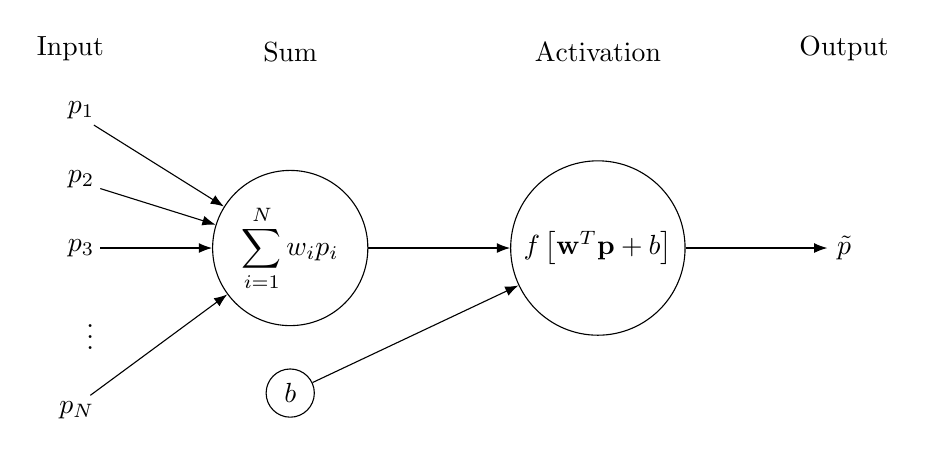
\begin{tikzpicture}[
node distance = 5mm and 18mm,
  start chain = going below,
  arro/.style = {-Latex},
bloque/.style = {text width=4ex, inner sep=2pt, align=right, on chain},
                        ]
% inputs
\foreach \i [count=\j] in {p_{1}, p_{2}, p_{3}, {\vdots}, p_{N}}
    \node[bloque] (in-\j) {$\i$};
% output
\node (out) [circle, draw, minimum size=6mm,
      %label=\textsc{$\displaystyle\sum_{i=1}^N$},
      right=of $(in-3)!0.5!(in-3)$]  {$\displaystyle\sum_{i=1}^Nw_ip_i$};
% conections
\foreach \i in {1,...,3}
    \draw[arro] (in-\i) -- (out);
\draw[arro] (in-5) -- (out);
% output
\node (output) [circle, draw, minimum size=6mm,right=of out]   
    {$f\left[{\bf w}^T{\bf p} + b\right]$};
%\coordinate[right=of out] (output);
\draw[arro] (out) -- (output);
% layer labels
\node[above=of in-1.center]     {Input};
\node[below=of in-4 -| out]     (bias) [circle,draw,minimum size=6mm]
                    {$b$};
\draw[arro] (bias) -- (output);
\node[above=of in-1 -| output]  {Activation};
\node[above=of in-1 -| out]  {Sum};
\node[right=of output] (final) {$\tilde p$};
\node[above=of in-1 -| final]  {Output};
\draw[arro] (output) -- (final);
\end{tikzpicture}
\caption{A model neuron, a constituent part of the artificial neural network model. The input from the previous layer ${\bf p}$ multiplied by corresponding weights ${\bf w}$ and summed. Then the bias $b$ is added, and the activation function $f$ is applied to the resulting ${\bf w}^T{\bf p}+b$. The output $\tilde p$ goes on to become input for neurons in the next layer. \label{fig:neuron}}
\end{centering}
\end{figure*}
The neuron is connected to the previous layers' neurons, and the strength of the connection is represented by a vector of weights, ${\bf w}$. Let us now consider a neuron which we will label by the index $k$. The output from neuron $i$ (of the preceding layer), $p_i$, is multiplied by the weight corresponding to the $i$\----$k$ connection, $w_i$. The combined weight vector multiplied by the input vector gives part of the total activation of the neuron, 
\begin{align}
\sum_{i=1}^Nw_ip_i = {\bf w}^T{\bf p}.
\end{align}
The remaining part is known as the bias, $b_k$. This is a single real number. There is one for each neuron, and it acts as modifier making the neuron more or less likely to fire independently of the input. 

The total input is passed to an activation (or transfer) function, which transforms it in some specified way, yielding the neuron \emph{output} $\hat p_k$. This in turn becomes input for the neurons in subsequent layers. 

Various different activation functions $f$ are used for different purposes. The function may be linear or non-linear, but should vanish for small inputs and \emph{saturate} for large inputs. For reasons that will become clear shortly, the conditions we enforce on $f$ is continuity, boundedness, as well as non-constantness. We also demand it be monotonically increasing. Numerous different transfer functions are in popular use today, and we will outline some of them in section \ref{sect:activations}.

In total, the action of a single neuron can be written
\begin{align}
\text{input}\ \rightarrow f\left({\bf w}^T{\bf p}+b\right) = \tilde p \ \rightarrow \ \text{output}.
\end{align}
A schematic representation of the single neuron connected to the previous and acting as input for the next layers is shown in \fig{neuron}. 

The full artificial neural network is built up of layers of neurons. Data is fed sequentially through the network, starting in the input layer (the input values can be thought of as the first layer), through the \emph{hidden} layers, and ending up in the output layer. The propagation needs to happen simultaneously across the network, as layer $k$ needs the fully computed output of layer $k-1$ before the activations can be calculated. 

A layer is\textemdash put simply\textemdash a collection of neurons, all of which are connected to the previous layer's neurons and the next layer's neurons. Let us label the individual neurons in layer $k$ by index $i$, i.e.\ $n_i^k$. The bias of neuron $i$ is then denoted $b^k_i$, and the weights connecting $n_i^{k-1}$ to $n_j^k$ is called $w_{ji}$. For each neuron there is a corresponding weight, so the weight vector is denoted $\bm{w}_i^k$. The combination of all weight vectors for layer $k$ thus makes a matrix, which we will denote by a capital $W^k$,
\begin{align}
W^k=\pmat{ccccc}{
  w^k_{11} & w^k_{12} & w^k_{13} & \dots & w^k_{1N} \\
  w^k_{21} & w^k_{22} & w^k_{23} & \dots & w^k_{2N} \\
  w^k_{31} & w^k_{32} & w^k_{33} & \dots & w^k_{3N} \\
  \vdots  &  \vdots   &   \vdots   & \ddots & \vdots \\
  w^k_{N1} & w^k_{N2} & w^k_{N3} & \dots & w^k_{NN}
}, \nonumber
\end{align}
or more compactly $(W^k)_{ij}=w^k_{ij}$. The collection of all biases for layer $k$ is $\mathbf{b}^k$. In this notation, we may write the propagation of the signal from layer $k-1$ to layer $k$ as 
\begin{strip}
\begin{align}
\mathbf{y}^k &= f(W^k\mathbf{y}^{k-1}+\mathbf{b}^k) 
=f\left( \bmat{ccccc}{
  w^k_{11} & w^k_{12}  & \dots & w^k_{1N} \\
  w^k_{21} & w^k_{22}  & \dots & w^k_{2N} \\
  \vdots  &  \vdots      & \ddots & \vdots \\
  w^k_{N1} & w^k_{N2}  & \dots & w^k_{NN}
} 
 \bmat{c}{y^{k-1}_1\\ y^{k-1}_2  \\ \vdots \\ y^{k-1}_N}  
+\bmat{c}{b^{k}_1  \\ b^{k}_2    \\ \vdots \\ y^{k}_N} \right) \label{eq:nnmatrix}
\end{align}
\end{strip}
or in Einstein notation (no sum over $k$ implied)
\begin{align}
y^k_i= f\big(w^k_{ij}y^{k-1}_j+b^k_i  \big).
\end{align}
In all of the preceeding three equations, application of $f$ indicates \emph{element wise} functional evaluation.

It is clear from \eq{nnmatrix} that propagation through an entire layer can be thought of as a matrix-vector product, a vector-vector summation, and a subsequent application of the transfer function $f$ element-wise on the resulting vector. 

A schematic representation of a layer consisting of three artificial neurons in a fully connected ANN is shown in \fig{layer}.

%Raff s. 51: "NN (and other non-linear black box techniques) cannot be expected to \emph{extrapolate} accurately."

\begin{figure*}
\begin{centering}
\def\layersep{4.5cm}
\begin{tikzpicture}[shorten >=1pt,->,draw=black!50, node distance=\layersep]
    \tikzstyle{every pin edge}=[<-,shorten <=1pt]
    \tikzstyle{neuron}=[circle,minimum size=17pt,inner sep=0pt]
    \tikzstyle{input neuron} =[neuron, draw=gray];
    \tikzstyle{output neuron}=[neuron, draw=gray];
    \tikzstyle{hidden neuron}=[neuron, fill=black];
    \tikzstyle{annot} = [text width=4em, text centered]

    % Draw the input layer nodes
    \foreach \name / \y in {1,...,3}
    % This is the same as writing \foreach \name / \y in {1/1,2/2,3/3,4/4}
        \node[input neuron, pin=left:{}] (I-\name) at (0,-\y) {};

    % Draw the hidden layer nodes
    \foreach \name / \y in {1,...,3}
        \path[yshift=0.0cm]
            node[hidden neuron] (H-\name) at (\layersep,-\y cm) {};

    % Draw the output layer node
  %\foreach \name / \y in {1,...,3}
    %    \path[yshift=0.0cm]
    %        node[hidden neuron] (H-\name) at (-\layersep,-\y cm) {};
    \node[output neuron,pin={[pin edge={->}]right:{}}, right of=H-3] (O) {};
    \node[output neuron,pin={[pin edge={->}]right:{}}, right of=H-3] at (\layersep,-1) (OO) {};
    \node[output neuron,pin={[pin edge={->}]right:{}}, right of=H-3] at (\layersep,-2) (OOO) {};

    
    % Connect every node in the input layer with every node in the
    % hidden layer.
    \foreach \source in {1,...,3}
        \foreach \dest in {1,...,3} 
            \path (I-\source) edge (H-\dest);
            

    % Connect every node in the hidden layer with the output layer
    \foreach \source in {1,...,3} {
        \path (H-\source) edge (O);
    \path (H-\source) edge (OO);
    \path (H-\source) edge (OOO);
    }

    % Annotate the layers
    \node[annot,above of=H-1, node distance=1cm] (hl) {Layer\ \ \ \ \ $k$};
    \node[annot,left of=hl]  {Layer\ \ \ $k-1$};
    \node[annot,right of=hl] {Layer\ \ \ $k+1$};
\end{tikzpicture}
\end{centering}
\caption{Schematic representation of a single ANN layer. Each neuron of the layer indexed $k$ is connected from behind to all neurons in layer $k-1$. The connection weights can be organized into a matrix, $W^{k-1}$, and the action of layer $k$ can be succinctly stated as $f(W^{k}{\bf p}^{k-1}+{\bf b}^k)$ where element-wise operation is assumed for the activation $f$. \label{fig:layer}}
\end{figure*}

\subsubsection{The full network}
A collection of $L$ layers connected to eachother forms a full \emph{network}. Note carefully that the network is nothing more than a (somewhat complex) function. If a single input and a single output value is specified, the action of the NN can be written out in closed form as 
\begin{strip}
\begin{align}
&\hat y\! = \!\left.\!\sum_{j=1}^{M}\! w_{1j}^L f_L\!\left(\!\sum_{k=1}^{M}\! w_{jk}^{L-1} f_{L-1}\!\left(\!
\sum_{i=1}^Mw_{ki}^{L-2} f_{L-2}\left( \dots f_1\!\Big(\!w_{m1}^1 x_1 \! + \!b_m^1\!\Big)
 \!\dots \!\right)+ b_i^{L-2}\right) \!+ \!b_k^{L-1}\!\right)
 \!+ \!b_1^L\!\right.. \label{eq:nnfull}
\end{align}
\end{strip}
Here, we have taken each layer to consist of $M$ neurons. The scalar $x_1$ denotes the input value, while $\hat y$ is the NN output. The transfer functions (which are \textit{not} assumed to all be the same) are denoted $f_L, f_{L-1},\dots,f_1$. From looking at \eq{nnfull}, the usefulness of the model is in no way obvious. But it turns out that for an ANN with at least one hidden layer populated with a finite number of neurons is a \emph{universal approximator} \autocite{HORNIK1989359}. This holds under the aforementioned assumptions on $f$. Being a universal approximator means (in this context) that the NN function can be made to be arbitrarily close to any continuous Borel-measurable function (essentially \emph{any} function we are likely to encounter) \autocite{mcdonald}. 

\subsection{Activation functions \label{sect:activations}}
Without any transfer functions, i.e.\ $f_l(x)=x$ for all layers $l$, the full network would simply be a linear transformation. In order to introduce non-linearities in our model, we employ one (or more) of a large set of possible activations. As mentioned, we require that these functions are continous and at least once (almost everywhere\footnote{A function with a property \textit{almost everywhere} (a.e.) denotes a function which satisfies this property everywhere, \textbf{except} possibly on a set of measure zero (such as e.g.\ a single point).}) differentiable, in order for the backpropagation scheme of section \ref{sect:backprop} to work. 

The following is an incomplete outline of activation functions in common use today. The simplest possible activation, the identity transformation $f_\text{I}(x)=x$, is commonly used for the output layer in regression networks. A simple (Heaviside) step function, $f_\text{H}(x)=H(x)$, with 
\begin{align}
f_\text{H}(x)=
\begin{cases}
1 & \text{ if } x\ge0 \\
0 & \text{ if } x<0 
\end{cases},
\end{align}
is sometimes used in the output layer of classification networks, but seldom in hidden layers because of the vanishing gradient making it impossible to train with backpropagation. The sigmoid function, 
\begin{align}
f_\text{S}(x)=\frac{1}{1+\mathrm{e}^{-x}},
\end{align}
is commonly used as hidden layer activations along with its sibling the hyperbolic tangent
\begin{align}
f_\text{t}(x)=\tanh(x)=\frac{\mathrm{e}^{x}-\mathrm{e}^{-x}}{\mathrm{e}^{x}+\mathrm{e}^{-x}}.
\end{align}
The tangent activation is a simple rescaling of the sigmoid, with $f_\text{t}(x)=2f_\text{s}(2x)-1$.

Simpler than the sigmoid, the family of activations known as \textit{rectifiers} consist of piecewise linear functions which are popular nowadays. The basic variant, the rectified linear unit (ReLU) is defined as 
\begin{align}
f_\text{ReLU}(x)=\max(0,x),
\end{align}
and is popular mostly because of its application to training \textit{deep} (many, large layers) neural networks\autocite{glorot2011deep}. Many variants of the ReLU exist, among the most well known are the leaky ReLU,
\begin{align}
f_\text{leaky ReLU}(x;\alpha)=
\begin{cases}
x & \text{ if }x\ge0 \\
\alpha x & \text{ if } x<0,
\end{cases}
\end{align}
the noisy ReLU
\begin{align}
f_\text{NReLU}(x) = \max(0,x+\mathcal{N}(0,\sigma)),
\end{align}
and the exponential linear unit
\begin{align}
f_\text{ELU}(x;\alpha) = 
\begin{cases}
x & \text{ if } x\ge 0 \\
\alpha(\mathrm{e}^x-1) & \text{ if } x< 0.
\end{cases}
\end{align}

\subsection{Training neural networks}
Knowing that ANNs can be universal approximators is not helpful unless we can find a systematic way of obtaining suitable parameters to approximate any given function $g(x)$. This is where \emph{training} comes in. Teaching a NN to approximate a function is conceptually simple, and involves only three steps:
\begin{shadeframe}
Assume input $x$ and corresponding \emph{correct} output $y$ is known.
\begin{itemize}
  \item[(1)] Compute output $\text{NN}(x)=\hat y$ of the artificial neural network, and evaluate the \emph{cost} function, $C(\hat y,y)$. 
  \item[(2)] Compute the gradient of $C(\hat y)$ w.r.t.\ all the parameters of the network, $w_{ij}^k$ and $b^k_j$.  
  \item[(3)] Adjust the parameters according to the gradients, yielding a better estimate $\hat y$ of the true output value $y$. 
  \item[(4)] Repeat (1)\textemdash(4).
\end{itemize}
\end{shadeframe}
The training scheme is known as \emph{supervised learning}, because the NN is continually presented with $x$, $y$ pairs, i.e.\ an input and an expected output. The cost (or objective or loss) function determines how happy the network is with it's own performance. In general, the output of the neural network is a vector of values, $\mathbf{y}$, and the cost function is taken across all outputs. In \eq{cost}, the network produces $N_\text{O}$ outputs for each input (which itself may be a vector). 

Step (3) is easy to understand, but complex in practice. In order to update the network weights and biases, a measure of the expected change in the total output is needed. Otherwise, any change would just be done at random\footnote{This is a possible approach, yielding a class of \emph{genetic} optimization algorithms. We will not discuss such schemes in the present work.}. This means we need to compute the set of derivatives 
\begin{align}
g_{ij}^k \equiv \frac{\partial C(\hat{\mathbf{y}})}{\partial w_{ij}^k}, \ \ \ \text{ and } \ \ \ h_i^k\equiv \frac{\partial C(\hat{\mathbf{y}})}{\partial b^k_i}.
\end{align}
The most common algorithm for computing these derivatives is the {\bf backpropagation} algorithm \autocite{backprop}. The method works by first pushing an input through the ANN, and computing the derivatives of the cost function w.r.t.\ the last layer weights and biases. The network is then traversed backwards, and the gradient w.r.t.\ all neuron parameters is found by repeated application of the chain rule. 

\subsection{Backpropagation \label{sect:backprop}}
Before we can apply the backpropagation algorithm, we need to perform a forward pass of the network given some input vector $\mathbf{x}\in\mathds{R}^{n_\text{f}}$, where $n_\text{f}$ denotes the number of features in the input data. We consider\textemdash for the moment\textemdash the case of a single input only ($n_\text{inputs}=1$). During the forward pass we calculate the activations $a^l$ of layer $l$, i.e.\ 
\begin{align}
a^l_j = f_l(z_j^l), 
\end{align}
where $z_j^l$ is the sum of a weighted sum of inputs from the previous layer and the bias of layer $l$, 
\begin{align}
z_j^1 = \sum_{i=1}^{n_\text{f}}w_{ij}^1x_i+b_j^1.
\end{align}
Assuming the layers have $N_l$ number of neurons, the calculated $z_j^l$ of subsequent layers takes the form
\begin{align}
z_j^l = \sum_{i=1}^{N_{l-1}}w_{ij}x_i+b_j^l,
\end{align}
where we note that $W^l\in\mathds{R}^{N_{l-1}\times N_l}$.

After performing the forward pass, we calculate the cost function and its derivative w.r.t.\ the weights in the output layer $W^L$,
\begin{align}
\frac{\partial C(W^L)}{\partial w_{jk}^L} &= \frac{\partial C(W^L)}{\partial a_j^L}\left[\frac{\partial a_j^L}{\partial w_{jk}^L}\right] \nonumber\\
%
&= \frac{\partial C(W^L)}{\partial a_j^L} \left[ \frac{\partial a_j^L}{\partial z_j^L}\frac{\partial z_j^L}{\partial w_{jk}^L} \right] \nonumber \\
%
&= \frac{\partial C(W^L)}{\partial a_j^L} f_L'(z_j^L)  a_k^{L-1}, \label{eq:deltaL}
\end{align}
where we used that (note $y_j=a_j^L$, i.e.\ the activations of the final layer)
\begin{align}
\frac{\partial C(W^L)}{\partial a_j^L} &= \frac{\partial }{\partial a_j^L} \left[\frac{1}{2}\sum_{i=1}^{N_\text{O}} (a_j^L-t_j)^2\right] \nonumber \\
&= a_j^L-t_j,
\end{align}
and 
\begin{align}
\frac{\partial z_j^L}{\partial w_{jk}^L} &= \frac{\partial}{\partial w_{jk}^L} \left[\sum_{p=1}^{N_L} w_{jp}^La_j^{L-1}+b_j^L\right] \nonumber \\
&= a_j^{L-1}. 
\end{align}

We define the quantity in \eq{deltaL} (apart from $a_k^{L-1}$ as $\delta_j^L$, meaning $\partial C/\partial w_{jk}^L=\delta^L_ja_k^{L-1}$. Applying the chain rule to $\delta^L_j$ yields the derivative of the cost function w.r.t.\ the output layer biases as
\begin{align}
\delta^L_j&= \frac{\partial C(W^L)}{a_j^L}\frac{\partial f^L}{\partial z_j^L} = \frac{\partial C(W^L)}{a_j^L}\frac{\partial a_j^L}{\partial z_j^L} \nonumber \\
%
&= \frac{\partial C(W^L)}{\partial z_j^L} = \frac{\partial C(W^L)}{\partial b_j^L} \frac{\partial b_j^L}{\partial z_j^L} \label{eq:deltad} \\
&= \frac{\partial C(W^L)}{\partial b_j^L},
\end{align}
where we used that 
\begin{align}
\frac{\partial b_j^L}{\partial z_j^L} &= \left[\frac{\partial z_j^L}{\partial b_j^L}\right]^{-1} \nonumber \\
%
&= \left[\frac{\partial}{\partial b_j^L} \sum_{i=1}^{N_{L-1}} w_{ij}^L a_i^{L-1}+b_j^L \right]^{-1} \nonumber \\
%
&= 1.
\end{align}
We have thus found the derivatives of the cost function w.r.t.\ both the weights and biases in the output layer, $W^L$ and $\mathbf{b}^L$. 

The equation 
\begin{align}
\delta_j^l &= \frac{\partial C}{\partial z_j^l}
\end{align}
holds for any layer, not just the output as in \eq{deltad}. Relating this to derivatives w.r.t.\ the layer $l+1$ $z_j$s, we find
\begin{align}
\delta_j^l &= \frac{\partial C}{\partial z_j^l} = \sum_k\frac{\partial C}{\partial z_k^{l+1}} \frac{\partial z_k^{l+1}}{z_j^l} \nonumber \\
&= \sum_k \delta_k^{l+1}\frac{\partial z_k^{l+1}}{z_j^l} \nonumber \\
%
&= \sum_k \delta_k^{l+1}w_{kj}^{l+1}\frac{\partial f^l}{\partial z_j^l}, \label{eq:backpropeq}
\end{align}
with 
\begin{align}
\frac{\partial z_k^{l+1}}{\partial z_j^l} &= \frac{\partial}{\partial z_j^l}\left[\sum_{i=1}^{N_l}w_{ik}^{l+1}a_k^l + b_k^{l+1}\right] \nonumber \\
%
&= \frac{\partial}{\partial z_j^l}\left[\sum_{i=1}^{N_l}w_{ik}^{l+1}f^l(z_k^l) + b_k^{l+1}\right] \nonumber \\
&= w_{jk}^{l+1}f^l(z_j^l).
\end{align}
The rest of the backpropagation scheme is essentially iterating \eq{backpropeq}, and computing\textemdash for each layer\textemdash the gradients $\partial C/\partial w_{ij}^l=\delta_i^la_j^{l-1}$ and $\partial C/\partial b_i^l=\delta_i^l$. Once the gradients are known, updating the weights and biases to improve the performance of the network (making the cost function smaller) can be done by e.g.\ gradient descent schemes, c.f.\ section \ref{sect:gradientdescent}.

\subsection{Exploding / vanishing gradients and weight initialization}
Typical transfer functions are constant or close to constant on most of $\mathds{R}$, and only changes appreciably in a tiny region around the origin. This means that a fully \textit{saturated} neuron with input $z_j\gg1$, or a \textit{dead} neuron with input $z_j\ll-1$ will most likely exhibit very small gradients and change very little durign training. This means the neurons are essentially wasted, they only add a constant input to the neurons in the subsequent layer; a job already performed by the bias $b_{j+1}$. In order to avoid this effect, it is important to initialize the weight matrices in the network in a smart way. 

In the useful region around the origin, we may assume that the transfer functions are roughly linear. In order for the signal to propagate through the network usefully, we essentially want the mean value of the $z_j$s to vanish, and the variance to be on the order of $1$. Let us now consider an input vector $X$ of $n$ components. If we take the weights to be random\textemdash as is the case in the first forward pass\textemdash then $W$ is a random vector of weights $W_i$. With the previous assumption about linearity of the transfer function, we get the activation 
\begin{align}
A=W_1X_1+W_2X_2+\dots+W_nX_n,
\end{align}
which has variance 
\begin{align}
\text{Var}(A) &= \text{Var}(W_1X_2+\dots+W_nX_n) \nonumber \\
%
&= n\text{Var}(W_i)\text{Var}(X_i),
\end{align}
where we assumed that the inputs and the weights are all independent, identically distributed, with vanishing mean. If we want the activation to have variance on the order of $1$, then we must require that the variance of the weights is 
\begin{align}
\text{Var}(W_i) = \frac{1}{n}.
\end{align}
Performing the same analysis with the backpropagated signal yields the same result,
\begin{align}
\text{Var}(W_i) = \frac{1}{n'},
\end{align}
with $n'$ being the amount of weights in the \textit{next} network layer. 

With this in mind,  Glorot \& Bengio suggested initializing weights with average variance:\autocite{glorot2010understanding}
\begin{align}
\text{Var}(W_i^l) = \frac{1}{n_l+n_{l+1}}.
\end{align}
In the case of sigmoid or hyperbolic tangent transfer functions, we may realize this variance by initializing $w=\mathcal{U}(-r,r)$ with
\begin{align}
r_\text{sigmoid}=\sqrt{\frac{6}{n_\text{in}+n_\text{out}}}, \nonumber \\
r_\text{tanh}=4\sqrt{\frac{6}{n_\text{in}+n_\text{out}}}, \nonumber
\end{align}
where $\mathcal{U}(a,b)$ denotes a uniform distribution between $a$ and $b$ and $n_\text{in}$ ($n_\text{out}$) is the number of neurons in the current (next) layer.

With rectifying linear units, the weight initialization scheme changes slightly. As the ReLU transfer function vanishes across half of $\mathds{R}$, He et al.\autocite{he2015delving} suggest doubling the variance of the weights in order to keep the propagating signal's variance constant, i.e.\
\begin{align}
\text{Var}(W)=\frac{2}{n_\text{in}}.
\end{align}
We may realize this by initializing weights $w=\mathcal{N}(0,1)\sqrt{2/n_\text{in}}$, where $\mathcal{N}(\mu,\sigma)$ denotes the normal distribution with mean $\mu$ and standard deviation $\sigma$.



\subsection{Gradient Descent \label{sect:gradientdescent}}
Almost every problem in machine learning and data science starts
with a dataset $X$, a model $g(\theta)$, which is a function of the parameters $\theta$ and a cost 
function $C(X, g(\theta))$ that allows us to judge how well the
model $g(\theta)$ explains the observations $X$. The model is fit by finding the values of $\theta$ that minimize the 
cost function. Ideally we would be able to solve for $\theta$ analytically, however this is not possible in general and 
we must use numerical methods to compute the minimum.
\subsubsection{The method of steepest descent}
The basic idea of gradient descent is that a function $F(\mathbf{x})$, $ \mathbf{x} \equiv (x_1,\cdots,x_n)$, 
decreases fastest if one goes from $\bf {x}$ in the direction of the negative gradient $-\nabla F(\mathbf{x})$.
It can be shown that if 
\begin{equation}
\mathbf{x}_{k+1} = \mathbf{x}_k - \gamma_k \nabla F(\mathbf{x}_k), \ \ \gamma_k > 0
\end{equation}
for $\gamma_k$ small enough, then $F(\mathbf{x}_{k+1}) \leq F(\mathbf{x}_k)$. This means that for a sufficiently 
small $\gamma_k$ we are always moving towards smaller function values, i.e a minimum. 

This observation is the basis of the method of steepest descent, which is also referred to as just gradient descent (GD). 
One starts with an initial guess $\mathbf{x}_0$ for a minimum of $F$ and compute new approximations according to
\begin{equation}
\mathbf{x}_{k+1} = \mathbf{x}_k - \gamma_k \nabla F(\mathbf{x}_k), \ \ k \geq 0.
\end{equation}
The parameter $\gamma_k$ is often referred to as the step length or the learning rate in the context of ML.

Ideally the sequence $\{ \mathbf{x}_k \}_{k=0}$ converges to a \textit{global} minimum of the function $F$. 
In general we do not know if we are in a global or local minimum.  
In the special case when $F$ is a \textit{convex function, all local minima are also global minima}, so in this case gradient 
descent can converge to the global solution. The advantage of this scheme is that it is conceptually simple and 
straightforward to implement. 

However the method in this form has some severe limitations:

\begin{itemize}
 \item In machine learing we are often faced with non-convex high dimensional cost functions with many local minimum. 
 Since GD is deterministic we will get stuck in a local minimum, if the method converges, unless we have a very good intial 
 guess. This also implies that the scheme is sensitive to the chosen initial condition.
 \item Note that gradient is a function of $\mathbf{x} = (x_1,\cdots,x_n)$ which makes it expensive to compute numerically.
 \item GD is sensitive to the choice of learning rate $\gamma_k$. This is due to the fact that we are only guaranteed 
that $F(\mathbf{x}_{k+1}) \leq F(\mathbf{x}_k)$ for \textit{sufficiently} small $\gamma_k$. The problem is to determine an 
optimal learning rate. If the learning rate is chosen to small the method will take a long to converge and if it is to 
large we can experience erratic behavior.
\item Many of these shortcomings can be alleviated by introducing randomness. One such method is that of Stochastic Gradient Descent 
(SGD).
\end{itemize}

\subsubsection{Stochastic Gradient Descent \label{sect:stochasticgradient}}
Stochastic gradient descent (SGD) and variants thereof address some of the shortcomings of the Gradient descent method discussed above. 

The underlying idea of SGD comes from the observation that the cost function, which we want to minimize, can almost always be 
written as a sum over $n$ datapoints $\{\mathbf{x}_i\}_{i=1}^n$,
\begin{equation}
 C(\mathbf{\theta}) = \sum_{i=1}^n c_i(\mathbf{x}_i, \mathbf{\theta}). 
\end{equation}
This in turn means that the gradient can be computed as a sum over $i$-gradients 
\begin{equation}
\nabla_\theta C(\mathbf{\theta}) = \sum_i^n \nabla_\theta c_i(\mathbf{x}_i, \mathbf{\theta}).  
\end{equation}
Now, stochasticity/randomness is introduced by only taking the gradient on a subset of the data called minibatches.  
If there are $n$ datapoints and the size of each minibatch is $M$, there will be $n/M$ minibatches. We denote these 
minibatches by $B_k$ where $k=1,\cdots,n/M$. 

As an example, suppose we have $10$ datapoints $( \mathbf{x}_1, \cdots, \mathbf{x}_{10} )$ and we choose to have $M=5$
minibathces, then each minibatch contains two datapoints. In particular we have 
$B_1 = (\mathbf{x}_1,\mathbf{x}_2), \cdots, B_5 = (\mathbf{x}_9,\mathbf{x}_{10})$. Note that if you choose $M=1$ you have 
only a single batch with all datapoints and on the other extreme, you may choose $M=n$ resulting in a minibatch for each 
datapoint, i.e $B_k = \mathbf{x}_k$.

The idea is now to approximate the gradient by replacing the sum over all datapoints with a sum over the datapoints in one the 
minibatches picked at random in each gradient descent step
\begin{align}\nabla_\theta C(\mathbf{\theta}) = &\sum_{i=1}^n \nabla_\theta c_i(\mathbf{x}_i, \mathbf{\theta}) \nonumber \\
\rightarrow &\sum_{i \in B_k}^n \nabla_\theta c_i(\mathbf{x}_i, \mathbf{\theta}).
\end{align}
                                                                                                                                                                                                 
Thus a gradient descent step now looks like 
\begin{equation} \theta_{j+1} = \theta_j - \gamma_j \sum_{i \in B_k}^n \nabla_\theta c_i(\mathbf{x}_i, \mathbf{\theta}) \end{equation}
where $k$ is picked at random with equal probability from the interval $[1,n/M]$. An iteration over the number of 
minibathces $n/M$ is commonly referred to as an epoch. Thus it is typical to choose a number of epochs and for each epoch 
iterate over the number of minibatches.
 
Taking the gradient only on a subset of the data has two important benefits. First, it introduces randomness 
which decreases the chance that our opmization scheme gets stuck in a local minima. Second, if the size of the 
minibatches are small relative to the number of datapoints ($M < n$), the computation of the gradient is much cheaper 
since we sum over the datapoints in the k-th minibatch and not all $n$ datapoints. 

A natural question is when do we stop the search for a new minimum? One possibility is to compute the full gradient after a 
given number of epochs and check if the norm of the gradient is smaller than some threshold and stop if true. However, 
the condition that the gradient is zero is valid also for local minima, so this would only tell us that we are close to a 
local/global minimum. However, we could also evaluate the cost function at this point, store the result and continue 
the search. If the test kicks in at a later stage we can compare the values of the cost function and keep the $\theta$ that 
gave the lowest value. 

Another approach is to let the step length $\gamma_j$ depend on the number of epochs in such a way that it becomes very small 
after a reasonable time such that we do not move at all. 

As an example, let $e = 0,1,2,3,\cdots$ denote the current epoch and let $t_0, t_1 > 0$ be two fixed numbers. Furthermore, 
let $t = e \cdot m + i$ where $m$ is the number of minibatches and $i=0,\cdots,m-1$. Then the function 
\begin{equation}\gamma_j(t; t_0, t_1) = \frac{t_0}{t+t_1} \end{equation}
goes to zero as the number of epochs gets large. I.e. we start with a step length $\gamma_j (0; t_0, t_1) = t_0/t_1$ which 
decays in "time" t. 

In this way we can fix the number of epochs, compute $\theta$ and evaluate the cost function at the end. Repeating the 
computation will give a different result since the scheme is random by design. Then we pick the final $\theta$ that gives 
the lowest value of the cost function.

\subsubsection{Gradient descent improvements: Adam}
While the stochastic gradient descent alleviates some of the problems intrinsic in the basic steepest descent method, it still has some problems. The \textit{stochasticity} allows it to possibly make jumps over small barriers, essentially transitioning into other basins of more optimal local minima. However, the SGD method struggles with navigating surfaces in parameter space in which the gradient is much steeper in one direction than the other(s). In this case, the iterations $\theta_i=(\alpha_i,\beta_i)$ will rapidly oscillate between over/under-shooting $\alpha_i$ values (with the steep gradient), while slowly making progress towards the minimum in $\beta_i$ (the shallow gradient).

We can help the SGD overcome this problem by introducing a \textit{momentum} term \autocite{qian1999monentum}. Instead of recomputing the gradient at each iteration, we keep a part of the change at the previous time step, essentially giving the optimization a momentum\textemdash accelerating the minimization in \textit{parameter space directions} in which the gradient is not steep, but consistently has a small value aimed steadily in one direction. It also hampers the rapid oscillating solutions in \textit{parameter space directions} in which we are close to the optimium, and the steep gradient makes the SGD over/under-shoot the solution at every other iteration. 

Each minibatch, the parameter update changes to
\begin{align}
\theta_{j+1} =\theta_j - \left[\eta \nabla_\theta c_i(\mathbf{x}_i,\theta_{j-1}) \right] - \gamma_j\nabla_\theta c_i(\mathbf{x}_i,\theta_j), \nonumber
\end{align}
with the momentum term $\eta$ usually set to a value close to $1.0$, e.g.\ $\eta=0.9$. The momentum term may be extended with a \textit{Nesterov accelerated gradient} scheme, which basically adds adaptive momentum term.

While introducing momentum into the SGD method improves the scheme, we are still disregarding a lot of previous\textemdash possibly relevant\textemdash information when we re-compute the gradient at each iteration and throw away all the history of previous gradients computed. In general, we should be able to use past moments of the calculated in previous iteration steps as a guide for the current gradient step in order to improve performance. This is exactly the motivation behind the Adam (Adaptive moment estimation) optimizer\autocite{kingma2014adam}.

\begin{algocf*}
\begin{shadeframe}
\begin{itemize}
  \item[] At step $j=0$, initialize $m_0=v_0=0$.
  \item[(1)] Iterate the step counter $j\leftarrow j+1$.
  \item[(2)] Calculate the gradient $g_j\leftarrow \nabla_\theta c(\mathbf{x}_i,\theta_j)$.
  \item[(3)] Update biased first moment estimate, \phantom{d}  $m_j\leftarrow \beta_1m_{j-1}+(1-\beta_1)g_j$.
  \item[(4)] Update biased second moment estimate, $v_j\leftarrow \beta_2v_{j-1}\phantom{d}+(1-\beta_2)g_j^2$.
  \item[(5)] Compute the bias-corrected first moment esimate, \phantom{d} $\hat m_j\leftarrow \frac{m_j}{1-\beta_1^j}$.
  \item[(6)] Compute the bias-corrected second moment esimate, $\hat v_j  \leftarrow \frac{v_j}{1-\beta_2^j}$.
  \item[(7)] Update parameter vector, $\theta_j\leftarrow \theta_{j-1} - \alpha \frac{\hat m_j}{\sqrt{\hat v_j} + \varepsilon}$.
\end{itemize}
\end{shadeframe}
\captionof{algocf}{The \textit{Adam} optimizer for stochastic optimization. The constants $\beta_1$, $\beta_2$, and $\varepsilon$ take appropriate default values $\beta_1=0.9$, $\beta_2=0.999$, and $\varepsilon=10^{-8}$. The initial step size $\alpha$ may be taken to be $0.001$. The gradient squared, $g_j^2$, denotes the elementwise square. \label{alg:adam}}
\end{algocf*}

The Adam scheme uses a moving, exponentially decaying, average of the first and second moments of the gradient to compute individual adaptive learing rates for each parameter independently. The moving average of the gradient $m_j$ is an estimate of the mean of the gradient, while the moving average of the gradient squared $v_j$ is an estimate of the (uncentered\footnote{The uncentered variance estimate of $\{f_i\}_{i=1}^N$, $\text{Var}_\text{u}(f)$ is the variance computed assuming $\langle f_i\rangle =0$, meaning the average is \textit{not} subtracted for each sample like usual,
\begin{align}
\text{Var}_\text{u}(f)&= \text{E}\left[\Big( f \Big)^2\right] \not= \text{E}\left[\Big( f - \langle f\rangle \Big)^2\right] = \text{Var}(f). 
\end{align}}) variance of the gradient. At the first iteration, we assign $m_0=v_0=0$, which means the estimates are inherently biased towards zero. In the Adam scheme, this is counteracted by computing bias-corrected estimates $\hat m_j$ and $\hat v_j$. The Adam optimization is outlined in algorithm \ref{alg:adam}.



\section{Model systems}
In this work we apply the machine learning algorithms discussed to the one- and two-dimensional Ising model. 
Linear regression and neural networks are used to estimate the coupling constant of the one-dimensional Ising model.

The two-dimensional Ising model is known to exhibit a first order phase transition at the critical \textit{Curie temperature}. In particular, the states of the model at sub-critical temperatures present as ordered, with large regions of spins aligned. At super-critical temperatures, the spins are disordered and essentially randomly uncorrelated. Thus it is interesting to investigate whether logistic regression or neural networks can be trained to to classify the phases. 

\subsection{The Ising model}
The Ising model can be thought of as a microscopic model of a ferromagnetic metal. The solid state metal exists in some energy-preferable lattice state\textemdash for simplicity, we assume a square lattice\textemdash and the magnetic dipole moments of the electrons due to their intrinsic spins are taken to occupy fixed positions on this lattice. In more complicated models (such as the Potts model\autocite{potts_1952}) the spins are allowed to take many different values, but in the basic Ising model the spins are restricted to being aligned either up or down ($+1$ or $-1$). The quantum mechanical exchange interaction energy between spins gives rise to the (no external magnetic field) simple model Hamiltonian for the system 
\begin{align}
H(\mathbf{s}) = -\sum_{i,j} J_{ij} s_is_j,
\end{align}
where $J_{ij}$ is the interaction energy matrix governing the size of the interaction between spins $i$ and $j$, while the state of the system (alignment of all spins) is denoted by $\mathbf{s}=\{s_i\}_{i=1}^N$. If $J_{ij}$ is positive, the energetically most efficient state of the system is realized if spins $s_i$ and $s_j$ are aligned in the same direction. Taking the total magnetization $\mathcal{M}$ to be the sum of all the spins (in the sense that spins aligned up are represented by $+1$, and downward facing spins are represented by $-1$), this $J_{ij}$ would facilitate spontaenous magnetization and thus model a ferromagnet. If $J_{ij}\le0$, the model system is a paramagnet (ideal paramagnet in the case of equality), giving rise to a $\mathcal{M}=0$ state unless an external field is applied.

The simplest case of \textit{nearest neighbor} interactions only is realized if $J$ takes the form
\begin{align}
J_{ij} = J_0\Big[\delta_{i,j+1} + \delta_{i,j-1} + \delta_{1,i}\delta_{j,N} + \delta_{N,i}\delta{j,0}\Big], \nonumber 
\end{align}
where the last term represents the periodic boundary conditions on $i$ and $j$. The $\delta$s here denote Kronecker deltas. We note that the constant $J_0$ must carry dimensions of energy per squared magnetic dipole moment. From now on we will assume $J>0$ in the rest of the project. 

An example of a 2D Ising lattice is shown in \fig{ising_lattice}.

The energetically most favorable state of the Ising lattice is one in which all spins are aligned either up or down. The energy of both \textit{all up} and \textit{all down} is the same\textemdash in the 1D case $E_\text{ground}=-NJ_0$\textemdash meaning there are two ground states. Assuming we put the spin model in thermal contact with a large heat bath at temperature $T$, but keep the number of spins and their occupied volume constant, we may write down the canonical partition function of the Ising model by considering every possible state of the lattice ($\mathcal{S}$) weighted by their respective Boltzmann factors,
\begin{align}
Z=\sum_{\mathbf{s}_k\in\mathcal{S}}\mathrm{e}^{-H(\mathbf{s}_k)/k_\text{B}T}.
\end{align}
Since flipping every spin in the lattice simultaneously does not affect the energy, there exists a \textit{flipped} version of every single state in $\mathcal{S}$ with the same energy and the same Boltzmann factor. When calculating canonical expectation values, the sum is taken over every possible state, so finding the expected magnetization of the Ising lattice will always yield zero since
\begin{align}
\langle \mathcal{M}\rangle &= \frac{1}{Z}\sum_{\mathbf{s}_k\in\mathcal{S}}\mathcal{M}(\mathbf{s}_k)\mathrm{e}^{-H(\mathbf{s}_k)/k_\text{B}T} \nonumber \\
%
&= \frac{1}{Z}\sum_{\mathbf{s}_k,\mathbf{s}_k'\in\mathcal{S}}\Big[\mathcal{M}_k-\mathcal{M}_{k'}\Big]\mathrm{e}^{-\beta E_k} = 0, \nonumber 
\end{align}
with $\mathcal{M}(\mathbf{s})=\mathcal{M}(\mathbf{s}')$ and $\mathbf{s}'$ representing the lattice state $\mathbf{s}$ with every single spin flipped. We here used $\beta=1/k_\text{B}T$ and defined $H(\mathbf{s})\equiv E_k$. Note that this is independent of the temperature.

\begin{figure}
  \centering
  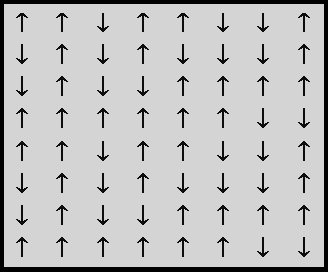
\includegraphics[width=0.8\textwidth]{ising_lattice.pdf}
  \caption{Example of a 2D square lattice of spins representing a (subset of a) full magnet. Counting the number of spins pointing up and the number pointing down yields $38$ total $\uparrow$s and $26$ $\downarrow$s, meaning we would in this case have a net magnetization in the $\uparrow$ direction. \label{fig:ising_lattice}}
\end{figure}

However, the two ground states both have $\mathcal{M}\not=0$. This constitutes a spontaneous symmetry breaking: When cooling the model from $T>T_\text{c}$ (the critical or \textit{Curie} temperature) to a temperature $T<T_c$, the magnetization will transition from a $\mathcal{M}=0$ state (super-critical, disordered) to an ordered $\mathcal{M}=\pm N$ ground state. At (or around) $T=T_c$ the energetic spin up/down symmetry is spontaneously broken, and the Ising lattice falls into one of the two possible ground states. This symmetry may be \textit{explicitly} broken by applying an external magnetic field $\mathbf{B}$, which adds a term $\propto \sum_{i=1}^N \mathbf{B}\cdot s_i$ to the Hamiltonian, breaking the $\mathbf{s}$\ce{<=>}$\mathbf{s}'$ symmetry.

An example of this symmetry breaking is visualized in \fig{metropolis}. Using the Metropolis algorithm to sample a pseudo-time evolution for a 2D Ising model with $N\times N$ spins, $N=1000$. Note that starting from a disordered state, the all-spins up ground state is randomly chosen by the system at $T<T_c$.

\begin{SCfigure*}
  \centering
  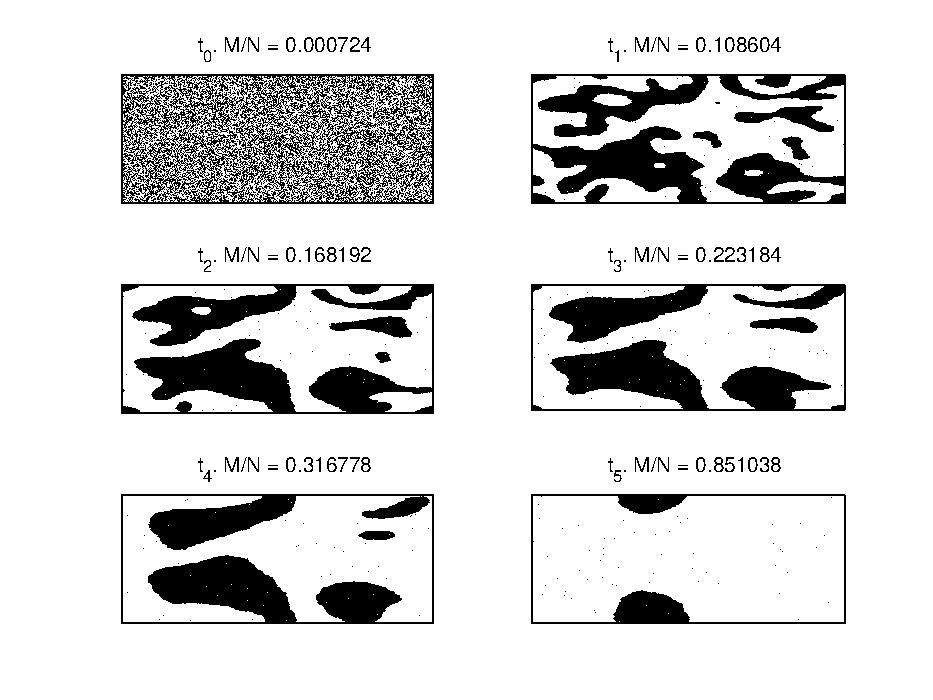
\includegraphics[width=0.45\textwidth]{ising_metropolis.pdf}
  \captionof{figure}{Results of application of the Metropolis algorithm to the Ising model with a randomized starting lattice. White pixels denote spin up, while black pixels denote spin down. The lattice used is $N\times N$ spins large, where $N=1000$. $t_i$ denote "time", i.e.\ the number of Monte Carlo cycles performed, but $t_i$ and $t_{i+1}$ are not necessarily equidistant for every $i$. $\mathcal{M}$ denotes the sum of all the spins ($1$ or $-1$) such that $\mathcal{M} / N^2$ is the relative magnetization of a single spin in the lattice. The temperature used was $1.2$ in units of $k_\text{B}T/J_0$, where $k_\text{B}$ is the Boltzmann constant. \label{fig:metropolis}}
\end{SCfigure*}

At the Curie temperature $T_c$, the 2D Ising model shows a second order \textit{phase transition}. Being a second order transition, the second derivatives of the free energy diverge. These include the spesific heat and the magnetic susceptibility,
\begin{align}
c_V &= \left(\frac{\partial E}{\partial T}\right)_{V,N} = -T\left(\frac{\partial^2 F}{\partial T^2}\right)_{V,N} \nonumber \\
\chi &= \left(\frac{\partial \mathcal{M}}{\partial B}\right)_{T,V}=\left(\frac{\partial^2 F}{\partial B^2}\right)_{T,V} \nonumber 
\end{align} 
The free energy $F$ here denotes the Helmholtz free energy.

\section{Results and discussion}
\subsection{Regression analysis on the one-dimensional Ising Hamiltonian \label{sect:1d_results}}
Since we have already validated the implementations of the linear regression methods in project 1, we go straight to the applications on the Ising model.

In the following we will take the 1D Ising model interaction matrix $J$ to be equal to
\begin{align}
J=J_0\pmat{cccccccc}{
  0 & 1 & 0 & 0 & \dots & 0 & 0 & 1 \\
  0 & 0 & 1 & 0 & \dots & 0 & 0 & 0 \\
  0 & 0 & 0 & 1 & \dots & 0 & 0 & 0 \\
  0 & 0 & 0 & 0 & \dots & 0 & 0 & 0 \\
  \vdots & \vdots & \vdots & \vdots & \ddots & \vdots & \vdots & \vdots \\
  0 & 0 & 0 & 0 & \dots & 0 & 1 & 0 \\
  0 & 0 & 0 & 0 & \dots & 0 & 0 & 1 \\
  0 & 0 & 0 & 0 & \dots & 0 & 0 & 0 \\
}
\end{align}
with $J_0=1$ being the coupling constant. We will start out by applying the regression schemes developed in project 1 to the 1D spin lattice and estimate the coupling constant $J_0$. We generate $N_s=1000$ sample lattice configurations (with the lattice size $L=40$) $\mathbf{s}_k$ and compute their energies as $H(\mathbf{s}_k)=\mathbf{s}_k^TJ\mathbf{s}_k$. For each configuration, we construct the design matrix by taking every possible combination of two spins multiplied. The rows of the design matrix take the following form
\begin{strip}
\begin{align}
\text{Row}_i(X) = \Big(s_1s_1, \,s_1s_2, \dots, s_1s_N,\, s_2s_1,\, s_2 s_2,\, s_2s_3, \dots, s_{N}s_{N-1},\, s_Ns_N \Big).
\end{align}
\end{strip}
The samples are split into a training set and a validation (test) set. We use a $50/50$ split, so the training set has size $N_t=500$ and the validation set has size $N_v=500$. The target data we fit against is the energy, $E_k$. Since the input is in the form of pairs of spins, we can directly interpret the found optimal $\beta$ parameters to be the full interaction matrix $J$. Inspired by the paper by Mehta et al.\autocite{mehta2018highbias}, we calculate the coefficient of determination, $R^2$ score, for the three different regression schemes, with varying degrees of regularization $\lambda$. This is shown in \fig{R2_lambda}. The reader is referred to the project 1 report for the definitions of the OLS/Ridge/Lasso schemes, $\lambda$, and the $R^2$ score.
\begin{SCfigure*}
  \centering
  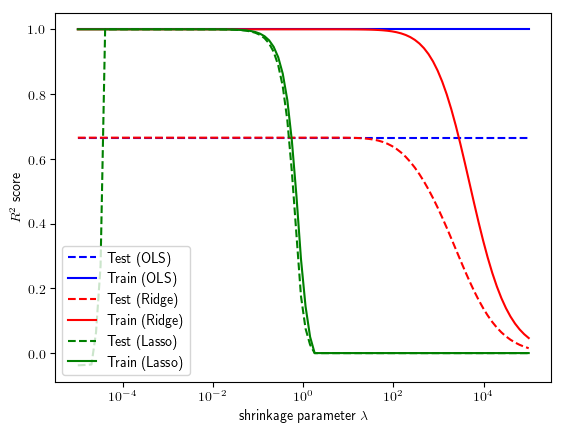
\includegraphics[width=0.52\textwidth]{R2_ising_lambda.png}
  \caption{Coefficient of determination, $R^2$ score, for the ordinary least squares, the Ridge, and the Lasso regression schemes applied to the 1D Ising model energy. Inspired by a similar figure in \cite{mehta2018highbias}. As expected, the OLS scheme outperforms the other methods on the \textit{training} set, but the Lasso regularization scheme is the only scheme which performs adequately on the validation set (for regularization parameter $\lambda$ in the range of approximately $10^{-1}$\textemdash$10^{-4}$).  \label{fig:R2_lambda}}
\end{SCfigure*}

Shown in the figure are the $R^2$ score as calculated from the training and the validation set for all three schemes. As expected, the OLS scheme is the best possible fit to the \textit{training} data. However, for a better gauge of overall model performance is the fit on untrained validation data. Here we see that the Lasso regression scheme with small regularization parameters dominates the other two methods. For $\lambda\sim10^{-1}$\textemdash$10^{-4}$ the Lasso scheme exhibits an $R^2\simeq 1$, while the OLS and Ridge methods fail to break $R^2\sim0.7$ across the entire broad range of $\lambda$ values tried. The ridge regression scheme performs worse than the OLS\textemdash on both the training \textit{and} validation sets\textemdash for $\lambda\gtrsim 10^2$. For smaller regularization parameters, the two are essentially indistinguishable. 

\begin{figure*}
  \centering
  \vspace{-1.5cm}
  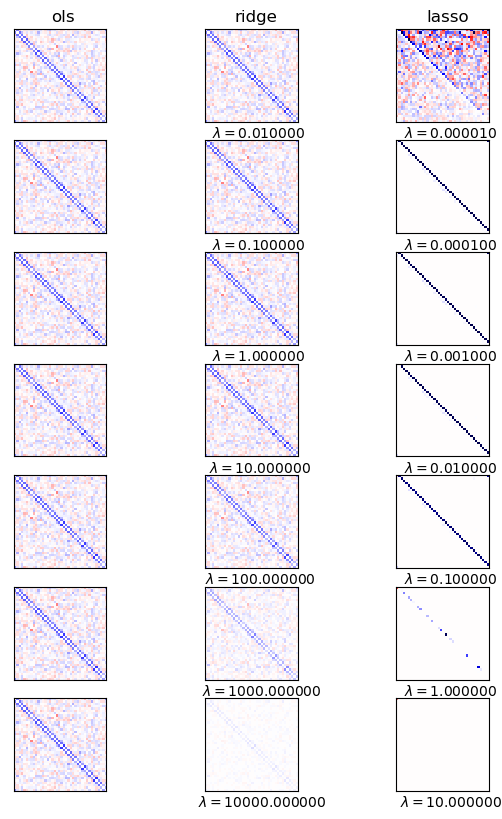
\includegraphics[width=0.8\textwidth]{1D_ising_beta_imshow.png}
  \caption{Visualizations of the $J$ matrix estimates gotten from the linear regression schemes discussed in section \ref{sect:1d_results}. The left column shows the OLS solution, the middle shows the Ridge regression solution, while the right hand side shows the interaction matrix as calculated by the Lasso regression scheme. Since the OLS method is independet of the regularization parameter $\lambda$, all the OLS matrices are equal. We note that in the OLS and Ridge cases, the a symmetric $J$ matrix is found, with values $0.5J_0$ on the $i=j+1$ and $i=j-1$ diagonals, while the input matrix only contains the upper $i=j+1$ diagonals. The latter is found by the Lasso scheme. Inspired by a similar figure in \cite{mehta2018highbias}. Please note carefully that the value of $\lambda$ used in the Ridge regression is three orders of magnitude larger than that of Lasso in each row of this figure.  \label{fig:imshow}}
\end{figure*}

As the optimized $\beta$ parameters can be interpreted as the estimated interaction matrix $J$, it is natural to visualize the form of the $\beta$ matrices for each method. This is shown in \fig{imshow}, where we perform fits for varying values of regularization $\lambda$. It is interesting to note that in the cases of OLS and Ridge regression, the solutions found exhibit a new symmetry that the input $J$ matrix does not. In the generated input data, only the upper $i=j+1$ diagonal of $J$ is populated with the values $J_0=1$. However, the computed energy is the same if we take $J$ to have both the $i=j+1$ and $i=j-1$ diagonals populated by $J_0/2$. This is what is found by the two mentioned schemes. The Lasso method, on the other hand, finds the single diagonal version of $J$ as it prefers performing variable selection\textemdash essentially zeroing out any unnecessary $\beta$s not absolutely needed\textemdash to find the optimal parameters.

The bias-variance tradeoff and the decomposition of the mean squared error into bias, variance, and irreducible error terms was discussed in project 1. We will not repeat the theory in the present work, but present in \fig{bias-variance} a bias-variance analysis of the linear models for varying regularization parameters $\lambda$. We use $k$-fold cross-validation with $k=10$ in order to extract the variance of the models. The reader is referred to the report for project 1 for a discussion about cross-validation. A system size of $L=40$ and $N=1000$ samples were used for all plots in \fig{bias-variance}. 

As expected, the sum of the bias squared and the variance equals the MSE for all models (to around machine precision). We will not introduce any noise in the current project, and thus our irreducible error vanishes. As the bias and variance of the OLS scheme does not depend on $\lambda$, that specific plot is ommitted. We note that as the regularization increases in strength, the bias increases. In general, it appears that the MSE of both Lasso and Ridge regressions are dominated by the bias term, except for very weak regularizations, $\lambda\sim10^{-5}$.

\begin{figure*}[p]
\centering
\subfloat[]     {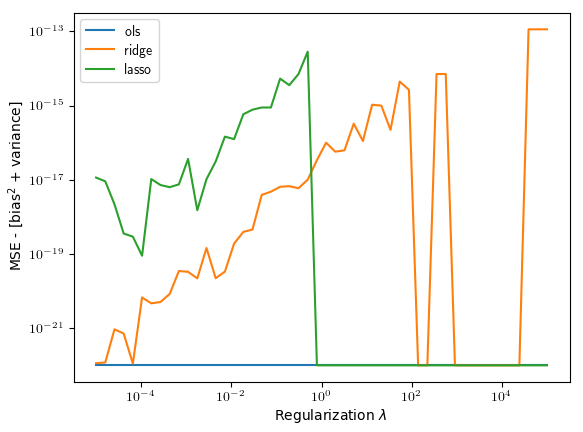
\includegraphics[width=0.8\linewidth]{bias-variance-1.png}} \\
\subfloat[Ridge]{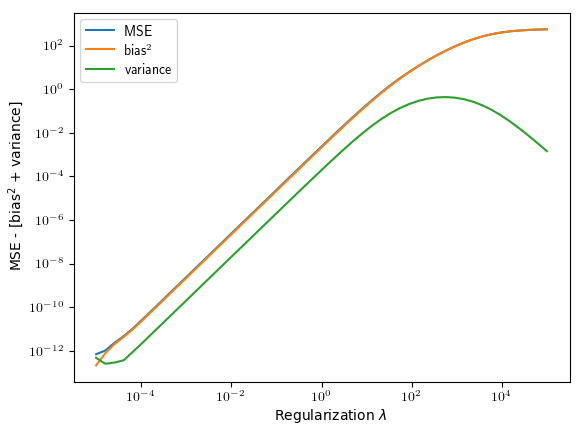
\includegraphics[width=0.5\linewidth]{bias-variance-ridge.png}}
\subfloat[Lasso]{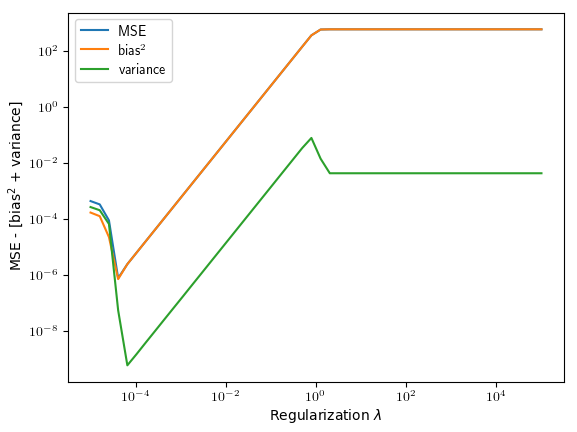
\includegraphics[width=0.5\linewidth]{bias-variance-lasso.png}}
\captionof{figure}{Absolute difference between the mean squared error and the sum of the bias squared and the variance in each model (top), and the individual MSE, bias, and variance for the Ridge and Lasso schemes (bottom). A system size of $L=40$ and $N=1000$ samples, with a $k$-fold cross-validation with $k=10$, were used to generate the data and extract the variance. Note the $y$-scale of the top plot, the $|\text{MSE}-(\text{bias}^2+\text{variance})|$ difference vanishes\textemdash despite the irregular appearance\textemdash to close to machine precision.  \label{fig:bias-variance}}
\end{figure*}


\subsubsection{Neural network regression}
We now turn our attention to regression analysis using neural networks. Training neural networks is a lot more tricky than optimizing linear regression models, so preparing our training samples requires a bit more finesse in this case. The statistical mechanical multiplicity of lattice states with net magnetization and energies close to $E,\mathcal{M}\sim0$ is \textbf{very} large compared the multiplicity of the ground state ($2$) and low/high $E,\mathcal{M}$ states. This means that if we just randomly generate $N$ arrays filled with $L$ values of $-1$ or $+1$, we will generate a vast majority of states with $E,\mathcal{M}$ close to zero, and almost no states with extreme $E\sim\pm J_0L,\mathcal{M}\sim \pm L$. This yields an inherent problem, as the NN can not be expected to approximate well sample states which it has only seen \textit{a few} times before in training. This problem of unbalanced training data can be solved easily in this case (but alas not in general, when generating new data is not as easy as pressing a button) by being smart about picking samples.

The ground state(s) have energy $-J_0L$, and changing any spin in a row of three aligned spins ($\uparrow\uparrow\uparrow\ \rightarrow \ \uparrow\downarrow\uparrow$ or $\downarrow\downarrow\downarrow\ \rightarrow\ \downarrow\uparrow\downarrow$) yields an energy difference of $\Delta E=4J_0$. The maximal energy state is the one in which alternating spins are always un-aligned, i.e.\ $\dots\uparrow\downarrow\uparrow\downarrow\uparrow\dots$, and this state has energy $+J_0L$. For $J_0=1$, that means there are $2L/4$ total possible energies for the 1D lattice. Starting in the \textit{maximal} energy state (which itself is doubly degenerate), we can generate a spin lattice of energy $J_0L-4J_0\mathcal{F}$ by flipping $\mathcal{F}$ of the even-indexed spins only. Note carefully that if we start with the ground state and flip $\mathcal{F}$ spins at random, we are in no way guaranteed to end up with a state of energy $-J_0L+4J_0\mathcal{F}$. In fact, this would only happen if you randomly picked only odd or only even numbered spins to flip, because otherwise you would perform at least one operation which would result in an energy difference $\Delta E\not=4J_0$ like e.g.\ $\uparrow\uparrow\downarrow\ \rightarrow \ \uparrow\downarrow\downarrow$ which gives an energy difference of $\Delta E=0$ (the two states are related by a flip of all three spins, and a left-right mirroring, neither of which affect the energy).

\newcommand{\ua}{ \ \uparrow \ }
\newcommand{\da}{ \ \downarrow \ }
Only in the case of starting from the maximal energy state and picking only odd or only even indexed spins to flip can we be sure to get a lattice of a specific energy. As an example, consider the $L=19$ example shown in the following, where we randomly pick $\mathcal{F}=3$ even numbered spins ($\downarrow$s) to flip. We denote the spins to be flipped by a $\bigodot$
\begin{strip}
\begin{align}
\text{Before: } &\ua \underset{\bigodot}{\da} \ua \da \ua \da \ua \underset{\bigodot}{\da} \ua \da \ua \da \ua \da \ua \underset{\bigodot}{\da} \ua \da \ua \da \ \ E=J_0L \nonumber\\
\nonumber\\
\text{After: } &\ua \ua \ua \da \ua \da \ua \ua \ua \da \ua \da \ua \da \ua \ua \ua \da \ua \da \ \ E=J_0(L-12)\nonumber\\
\end{align}
\end{strip}
We flipped the three spins with indices $2$, $8$, and $16$ and ended up with a $\Delta E=3\cdot 4J_0$. Preparing $N/2$ such samples in the before state, and then iterating over $\mathcal{F}=0,1,2,\dots,L/2$, applying $\mathcal{F}$ even indexed random spin flips to $N/L$ of the $N/2$ total samples will yield bins of $N/L$ random configurations all with energies $E=J_0(L-4\mathcal{F})$. For the other $N/2$ samples, we start off with the \textit{other} maximal energy state (all spins flipped), and instead flip successively $\mathcal{F}$ even indexed\textemdash but now $\uparrow\ \rightarrow \downarrow$ instead of the opposite\textemdash to not bias the sampling towards one class of configurations. All in all, this yields a set of $N$ samples with even probabilities to take on any of the $2L/4$ possible energies. In contrast, sampling in the naive but simple way overwhelmingly yields samples in the range around $E\sim0$. Illustrating this, the cumulative probability of picking a random sample with energy $E$ out of the sample set for both versions of the data set generation is shown in \fig{cdf}. We call the method of sampling outlined in this section \textit{even sampling}. In this plot, a $L=1000$ lattice is sampled $N\approx1000$ times. A similar effect (though less extreme) is exhibited by smaller grids. 

\begin{figure}
  \centering
  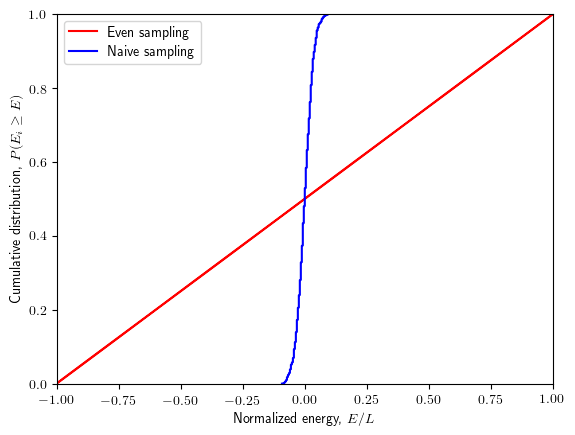
\includegraphics[width=\textwidth]{visualize_sampling.png}
  \caption{Cumulative probability density function for picking a random sample with energy $E_i$ out of the total data set, for the straight forward sampling method and the even sampling described in section \ref{sect:1d_results}. Note that a linear cumulative distribution means the probability density is flat, i.e.\ uniform probability. The naively generated data set exhibits a probability density function sharply peaked around $E=0$. \label{fig:cdf}}
\end{figure}

Having devised a method of sampling states which will be helpful for the NN training, we move on to the training. First off, we prepare networks with $L$ inputs, a single hidden layer of $L^2$ neurons, and an output with identity activations. For the moment, we use sigmoid activations for the hidden layer. We prepare a data set of $N=5000$ lattice configurations of \textit{evenly} sampled energies, and reserve $N_v=1000$ of them for validation purposes. The Adam optimizer is run for a total of $1000$ epochs, with a batch size of $1000$, and an initial step size $\alpha=0.001$. The mean squared difference between the target energies and the NN output is used as the cost function for training with the bakcpropagation algorithm. For varying lattice sizes $L=10,\dots,40$ we perform the fit and visualize the output. This is shown in \fig{NN_out}. Note that the energies are normalized (divided by $L$) and take values in $[-1,1]$, to help the NN during training. 

\begin{figure*}[p]
\centering
\subfloat[$L=10$]{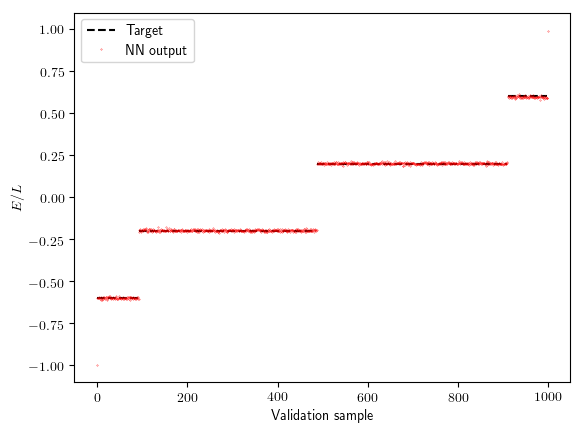
\includegraphics[width=0.5\linewidth]{nn_1d_energy_predict10.png}}
\subfloat[$L=20$]{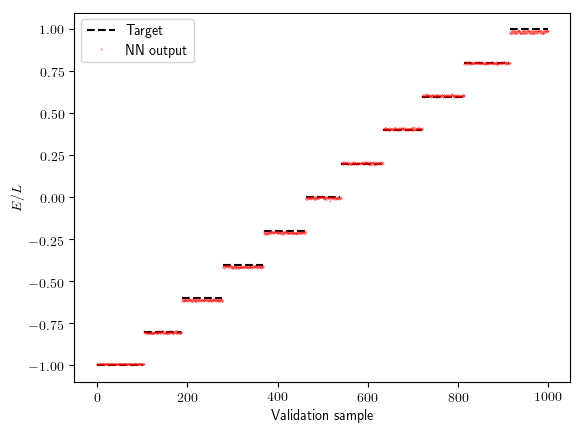
\includegraphics[width=0.5\linewidth]{nn_1d_energy_predict20.png}} \\[-10pt]
\subfloat[$L=30$]{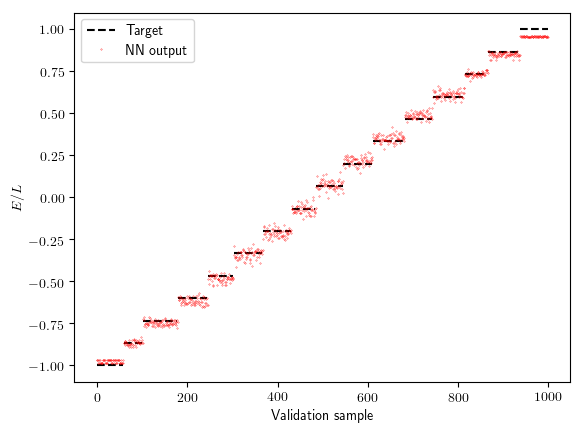
\includegraphics[width=0.5\linewidth]{nn_1d_energy_predict30.png}}
\subfloat[$L=40$]{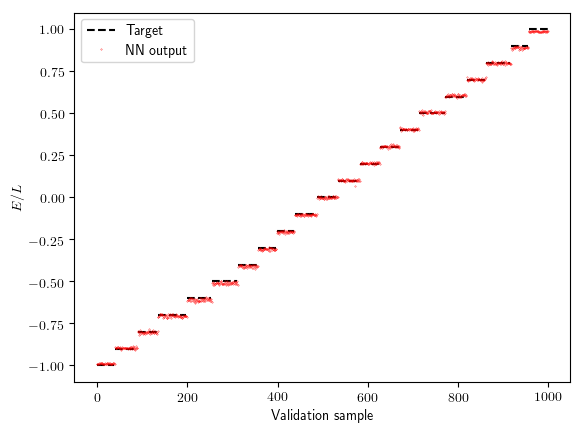
\includegraphics[width=0.5\linewidth]{nn_1d_energy_predict40.png}}
\captionof{figure}{Raw NN output and target validation energies for different lattice sizes after training for $1000$ epochs with a data set of $N=5000$ samples. The energies are normalized by $L$. We note that the NN output roughly follows the true target, but more training is necessary to reach very good results.\label{fig:NN_out}}
\end{figure*}

% Training 5000  epochs L=5:         36.547 s
% Training 10000 epochs L=10: 3  min 37.836 s
%          10000 epochs L=15: 4  min 19.580 s
%          20000              10 min 41.648 s
%          20000        L=20: 19 min 23.448 s
%          20000        L=25: 34 min 48.781 s
%          20000        L=30: 54 min  4.239 s

\begin{SCfigure*}
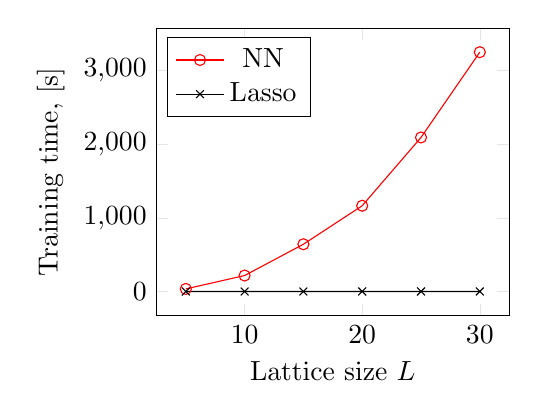
\begin{tikzpicture}
  \begin{axis}[
    width=0.5\textwidth,
    xlabel=Lattice size $L$,
    ylabel={Training time, $[\text{s}]$},
    legend pos=north west]
  \addplot[color=red,mark=o] coordinates {
    (5,    36.547)
    (10,  217.836)
    (15,  641.648)
    (20, 1163.448)
    (25, 2088.781)
    (30, 3244.239)
  };
  \addlegendentry{NN} 
  \addplot[color=black,mark=x] coordinates {
    (5,   1.527)
    (10,  1.680)
    (15,  1.771)
    (20,  1.793)
    (25,  2.153)
    (30,  2.190)
    %(50,  2.443)
    %(100, 5.089)
  };
  \addlegendentry{Lasso} 
  \end{axis}
\end{tikzpicture}
\captionof{figure}{Training time for the regression neural networks trained to estimate the energy of 1D Ising lattice configurations for different system sizes $L$. Even though the NN may outperform the linear schemes in terms of the mean squared error on a validation set\textemdash for small $L$\textemdash it is hard to justify the cost\textendash benefit ratio in terms of training time required. The Lasso time peaks at around $2\,\text{s}$. \label{fig:time}}
\end{SCfigure*}

From the plots in \fig{NN_out}, it is pretty clear that our trained networks leave a lot to be desired. One remedy it increasing the data set size for training, and increasing the training time (number of epochs). In order to compare against the linear regression models we discussed earlier, we investigate now how much training is necessary in order to surpass the performance of the Lasso regression at $\lambda=10^{-2}$. This was deemed the best of the linear methods earlier. 

We consider small enough system sizes $L$ for the training to be feasible (training time on a late\textendash2013 MacBook pro running OSX10.11.6 approximately less than 60 minutes), and keep going until the MSE has reached an apparent plateu. Comparing the mean squared error of the trained NN against the $\lambda=10^{-2}$ for varying small lattices is shown in \fig{NN_lattice}. It is clear that in some cases, the NN scheme is able to surpass the performance on the validation sets. However, as the lattice grows in size, the required training time becomes unfeasible, as shown in \fig{time}. It is hard to justify an order of magnitude or two drop in MSE at the cost of over $1500$ times increase(!) in preparation time (the Lasso scheme does not require more than at most $2.2\,\text{s}$ for even the largest of these lattices). 

\begin{figure*}[p]
\centering
\subfloat[$L=5$] {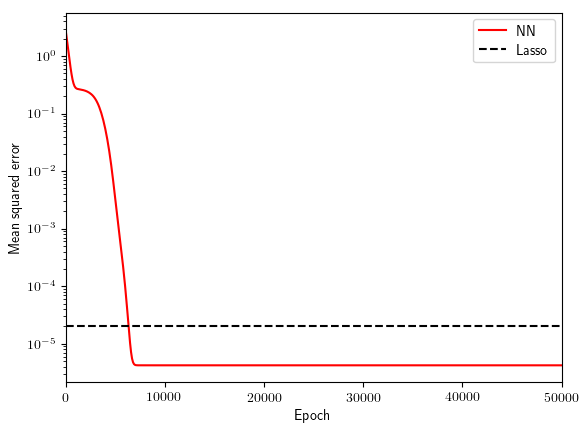
\includegraphics[width=0.5\linewidth]{NN_compare_lasso5_2.png}}
\subfloat[$L=10$]{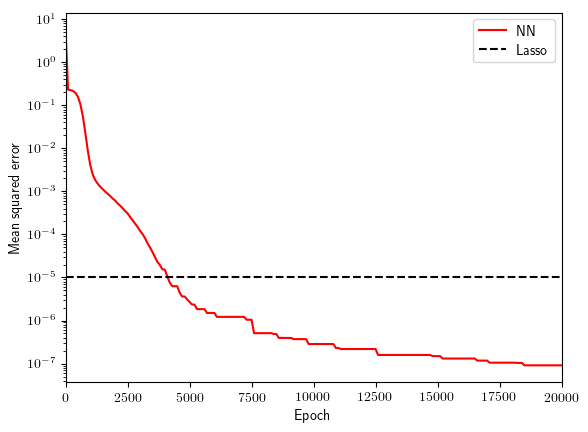
\includegraphics[width=0.5\linewidth]{NN_compare_lasso10_2.png}} \\[-10pt]
\subfloat[$L=15$]{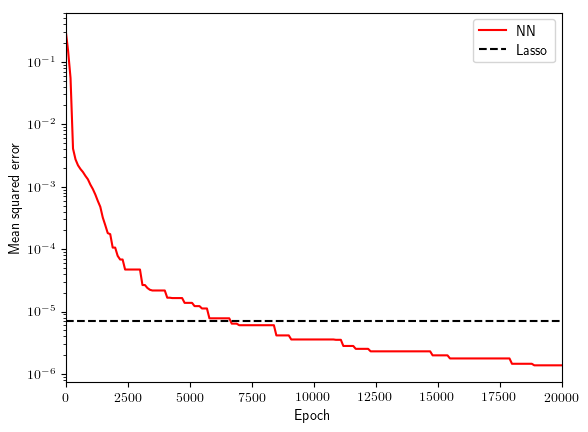
\includegraphics[width=0.5\linewidth]{NN_compare_lasso15_2.png}}
\subfloat[$L=20$]{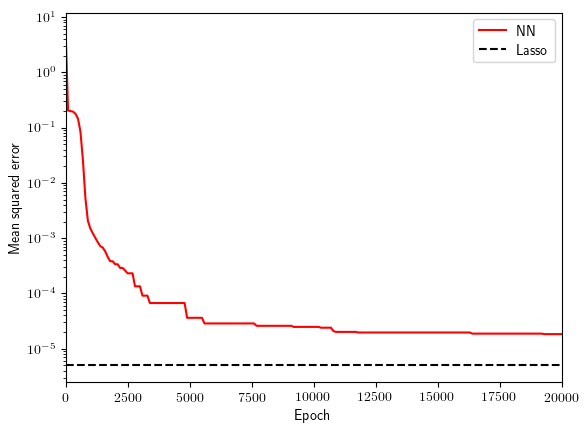
\includegraphics[width=0.5\linewidth]{NN_compare_lasso20.png}} \\[-10pt]
\subfloat[$L=25$]{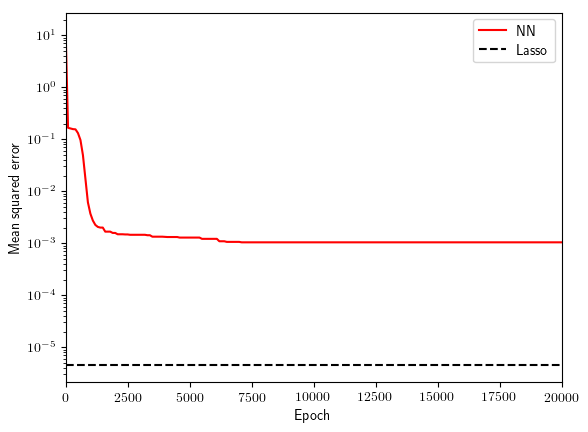
\includegraphics[width=0.5\linewidth]{NN_compare_lasso25.png}}
\subfloat[$L=30$]{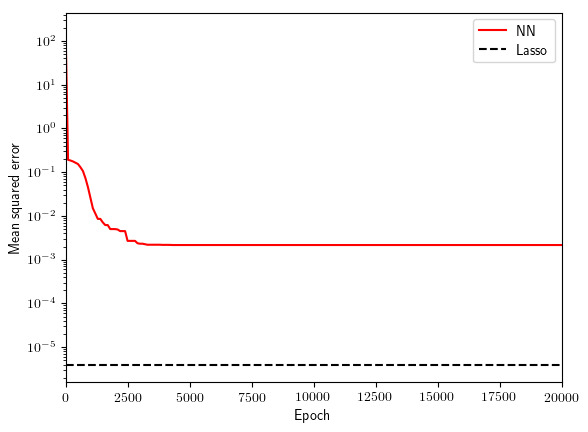
\includegraphics[width=0.5\linewidth]{NN_compare_lasso30.png}}
\captionof{figure}{Mean squared error calculated from trained networks applied to small\textendash medium sized Ising lattices. We note that for sufficiently small system sizes, the NN outperforms the Lasso scheme (which was shown to be the best performer of the linear models). However, as the lattice growns, the training time required either makes training unfeasible or the training is simply not able to reduce the MSE to below that of the Lasso scheme (a plateu is hit before the NN performance surpasses that of the Lasso method). The training time for each network is shown in \fig{time}. \label{fig:NN_lattice}}
\end{figure*}

\newcommand{\sym}{\text{Sym}\,}
\renewcommand{\skew}{\text{Skew}\,}
\subsubsection{Recovering the $J$ matrix in the neural network model}
As a closing remark for the neural network regression section, we note the apparent difficulty of recreating the $J$ matrix using the neural network scheme. Even using identity activations, the design matrix as network input (each sample being $L^2$ values of every combination of $s_is_j$) and a single hidden layer with one neuron (making the first network weight $L\times L$), and freezing the intercepts at $0$, we are still not able to recreate the $J$ matrix. As an example, training a $L=5$ model like this yields an MSE that vanishes to machine precision ($\sim10^{-30}$), however the resulting weight matrix takes the form:
\begin{align}
W\approx
\pmat{ccccc}{
 0.59 & -1.77 &  0.18 &  0.22 &  0.83 \\
 0.81 & -0.14 & -1.65 & -0.39 & -0.72 \\
-0.18 &  0.69 & -0.85 & -0.48 & -0.52 \\
-0.22 &  0.39 & -0.48 &  0.81 & -1.03 \\
-1.79 &  0.72 &  0.52 &  0.07 & -0.41
} \nonumber
\end{align}
It is not at all obvious why this matrix should yield essentially zero error in the energy for every single $L=5$ state available. In order to make sense of this, we note a \textit{key observation}: The energy is given by the quadratic form $\mathbf{s}^TJ\mathbf{s}=E$ and any quadratic form $\mathbf{x}^TA\mathbf{x}$ is invariant under the exchange of $A$ and the symmetric part of the matrix, $(A+A^T)/2$. As an example of this, the symmetric part of the standard $J$ interaction matrix used so far in the present work is (zeros ommitted)
\begin{align}
\hspace{-1cm}\frac{J+J^T}{2}&=-\frac{1}{2}\pmat{ccccccc}{
   & 1 &   &   &   &   &  1\\
 1 &   & 1 &   &   &   &   \\
   & 1 &   & 1 &   &   &   \\
   &   & 1 &   &   &   &   \\
   &   &   &   & \ddots & & \\
   &   &   &   &   &   & 1 \\
 1 &   &   &   &   & 1 &  
},\label{eq:symj}
\end{align}
which we have already discussed: This is is the symmetric version found by the OLS and Ridge regression methods. In the following, we denote the symmetric part of a square matrix $A$ by
\begin{align}
\sym A=\frac{A+A^T}{2},
\end{align}
while the remaining, non-symmetric, part of $A$ is called the \textit{skew}-symmetric (or anti-symmetric) part of $A$,
\begin{align}
\skew A=\frac{A-A^T}{2}.
\end{align}
Note that $A=\sym A+\skew A$, with $(\sym A)^T=\sym A$ and $(\skew A)^T=-\skew A$.

As the aforementioned $W$ matrix recovers the energy to machine precision, that must necessarily mean that $\mathbf{s}^TW\mathbf{s}=\mathbf{s}^TJ\mathbf{s}=E$. Computing the symmetric part of $W$ yields an interesting result:
\begin{align}
\sym W&=-\frac{1}{2}\pmat{ccccccc}{
D_1'& 1 &   &   & 1  \\
 1 &D_2'& 1 &   &    \\
   & 1 &D_3'& 1 &    \\
   &   & 1 &D_4'& 1  \\
 1 &   &   & 1 & D_5'
}\nonumber \\
&= \sym J + D. \label{eq:wsym}
\end{align}
As we can see, we are tantalizingly close to recreating the symmetric part of $J$\textemdash the only difference is the diagonal elements, which we may organize in a matrix $D$ with elements\footnote{The $D_i$ and the $D_i'$ elements shown in \eq{wsym} are related by $D_i=-D_i'/2$, where we simply absorbed the constant into $D_i'$ for ease of notation.} $D_i$. It is obvious that since the original equation $\mathbf{s}^TW\mathbf{s}=\mathbf{s}^TJ\mathbf{s}$ holds, and any quadratic form is invariant under a $A\mapsto \sym A$ transformation, then 
\begin{align}
E&=\mathbf{s}^T W\mathbf{s}\nonumber \\
&=\mathbf{s}^T\sym W\mathbf{s}\nonumber \\
&=\mathbf{s}^T(\sym J + D)\mathbf{s} \nonumber \\
&=\mathbf{s}^T\sym J \mathbf{s} + \mathbf{s}^T D\mathbf{s} \nonumber \\
&= E + \mathbf{s}^T D\mathbf{s}\label{eq:esym}
\end{align}
which can only be true if $\mathbf{s}^TD\mathbf{s}=0$. In general, quadratic forms are not invariant under $A\mapsto A+D$, with $D$ a diagonal matrix. However, in our special case\textemdash recall that the input state can only take values $s_i=\pm 1$\textemdash it is, if and only if $\text{Tr}\,D=0$. 

To see that this is the case, consider the $D$ term of \eq{esym}, which itself is a quadratic form
\begin{align}
\mathbf{s}^TD\mathbf{s}=\sum_{i=1}^L s_i s_i D_i,
\end{align}
and note that this corresponds to self-interaction in the Ising lattice (spin $i$ interacting with spin $i$, itself). Since $s_i^2=1$ for any $s_i\in\{-1,1\}$, we find that
\begin{align}
\mathbf{s}^TD\mathbf{s}=\sum_{i=1}^L s_i^2D_i = \text{Tr}\,D.
\end{align}
Of course, the $W$ matrix found by our neural network has vanishing trace, explaining how it is able to recover the energy perfectly. 

In general, any regression scheme (linear or NN-based or otherwise) is not concerned with recovering the matrix $J$, but rather with finding any matrix $A$ in the class of $L\times L$ matrices, which satisfy
\begin{align}
\Big\{A\in &\mathds{R}^{L\times L}\,:\,\sym A=\sym J+D, \nonumber \\
& D=\text{diag}(D_1,\dots,D_L), \,\text{Tr}\,D=0 \Big\}.
\end{align}


%It is hard to say why and how this matrix should yield essentially exactly correct energies for all $2000$ samples in the validation set, and we can offer no insight into the mechanism at work here. However, we find that $\mathbf{s}_k^T W \mathbf{s}_k=\mathbf{s}_k^T J \mathbf{s}_k$ to machine precision. 

This whole ordeal outlines a fundamental difficulty in working with machine learning algorithms such as the present one; it is essentially a \textit{black box}. Even when it works perfectly, understanding \textit{why} or \textit{how} it works may involve a considerable amount of effort.

Finally we note a curiosity: The $\text{Tr}\,D=0$ demand is simply an artifact of the way we train the model. If we add a constant $\alpha$ to all energies when training, $E\mapsto E+\alpha$, we would recover it as $\text{Tr}\,D=\alpha$. Physically, a constant shift in the energy has no impact on the dyanamics of a system, and physically nothing prevents us from adding such terms. In the Ising model, we could interpret the self-interaction of spin $s_i$ as the \textit{self-energy} of spin $i$, i.e.\ the energy necessary for spin $s_i$ to simply exist in the lattice regardless of it's interaction with the other spins.


\subsection{Classifying phases of the two-dimensional Ising model \label{sect:ising2d}}

We consider the 2D Ising model on a $40 \times 40$ lattice. There are three possible types of states: ordered $T/J < 2.0$, 
critical $2.0 \leq T/J \leq 2.5$ and disordered $ T/J > 2.5$.

Mehta et al.\autocite{mehta2018highbias} 
have made avaiable a data set where Monte Carlo sampling is used to prepare $10^4$ states at sixteen uniformly spaced 
temperatures $T/J \in [0.25,4.0]$. 

Each data point is represented by a state-vector 
\begin{equation}
 \mathbf{x}^{(i)} = (s_1, \dots,s_{1600}), \ \ s_k \in \{-1,+1\}
\end{equation}
and a label $y_i \in \{0,1\}$ with $y_i = 1$ corresponding to an ordered state.


\subsubsection{Logistic regression analysis on the two-dimensional Ising model}
The logistic regression model is trained using a set of ordered and disordered states, while the critical states are left out. 
This training set is split 50/50 in a training and test set. When the training procedure is finished, the performance of 
the model is measured on both the test set and the set of critical states not used in the training phase. 

In Fig.\ref{MehtaComparison} we have computed the training, test and critical accuracy for regularization parameters 
$\lambda \in [10^{-5},10^{5}]$. The results are in excellent agreement those obtained by Mehta using scikit-learn's \textit{logistic regression}
functionality \footnote{\href{https://scikit-learn.org/stable/modules/generated/sklearn.linear\_model.LogisticRegression.html}{https://scikit-learn.org/}}.

For small $\lambda$ we observe that the accuracies are essentially unaffected by the regularization strength. 
However for $\lambda$ roughly in the range $10-100$ we see a slight increase in the critical accuracy while the training and 
test accuracy stays the same. On the other hand, for large $\lambda$ we observe an increasing critical accuracy at the cost of 
decreasing training and test accuracy. 

Furthermore, we note that in general the model seems to perform roughly $10$\% worse on 
the critical states compared with the ordered and disordered states.  

Another observation is that if the logistic model is trained without an intercept term, we end up with a result 
which is essentially guessing as shown in Fig.\ref{logRegNoIntercept}.

\begin{figure}[h!]
\centering
 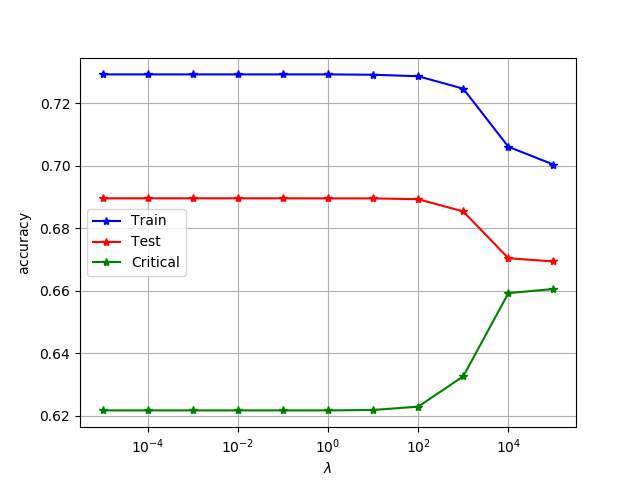
\includegraphics[width=1\linewidth]{logReg_acc_vs_regstrength_Final.png}
 \captionof{figure}{Training, test and critical accuracy plotted as function of regularization parameter $\lambda$. 
 We remark that for small $\lambda$ the accuracies are essentially unaffected by the regularization. However for $\lambda$ roughly in 
 the range $10-100$ we see a slight increase in the critical accuracy while the training and test accuracy stays the same. On the 
 other hand, for large $\lambda$ we observe an increasing critical accuracy at the cost of decreasing training and 
 test accuracy.}
 \label{MehtaComparison}
\end{figure}

\begin{figure}[h!]
\centering
 %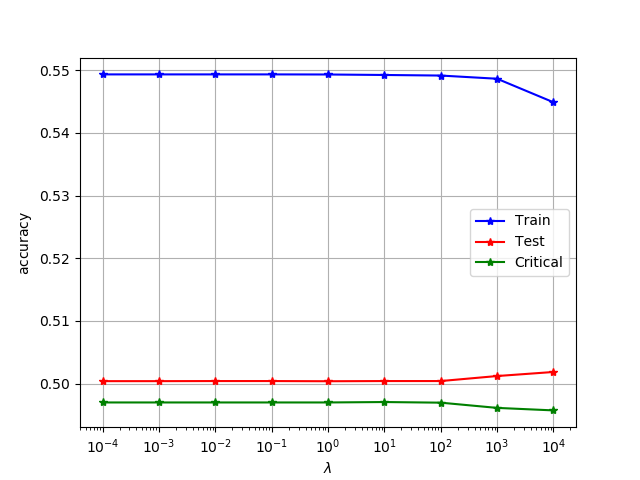
\includegraphics[width=1\linewidth]{logReg_acc_vs_regstrength_noIntercept.png}
 \captionof{figure}{Training, test and critical accuracy plotted as function of regularization parameter $\lambda$ without 
 intercept term. We clearly see that the training, test and critical accuracies are close to 50\%, i.e. we end up with 
 a sophisticated way of wild guessing. 
 }
 \label{logRegNoIntercept}
\end{figure}

\subsubsection{Classification using the neural network model}
Lastly, we turn to classification of the 2D Ising model ordered/disordered states, described in section \ref{sect:ising2d}, using a neural network model. Classification is done with a softmax cross-entropy activation/cost function combo in the last layer of the network, while we retain the sigmoid activations for the earlier layer(s). The network architecture used consists of a single hidden layer of $100$ neurons, feeding into a layer of a single neuron (the softmax activation) and the two outputs (in one-hot vector format). As no regularization was necessary to obtain satisfactory results, $\lambda=0$ was used throughout this section. We use the Adam optimizer, and a batch size of $2000$ states. 

As the entire data set is rather large, our first attempt takes only a random subset of $20\,000$ total configurations for training (roughly a third of the Mehta data). Half of the $20\,000$ are used for training, the other half are used for validation. In addition, we use the separate samples around $T_c$ for secondary validation. Training for $2000$ epochs yields an acceptable accuracy, as shown in \fig{nn_accuracy_20k}. Note that $1-\text{accuracy}$ is shown, i.e.\ lower is better. The peak accuracy reached on the training samples was $99.89\%$, while the accuracy on the validation set was $98.86\%$. On the $30\,000$ samples around the Curie temperature, the accuracy attained was $94.50\%$, meaning $1652$ of the $30\,000$ were misclassified. This is already impressive compared to the logistic regression scheme, but we can do better.


\begin{figure}
\centering
 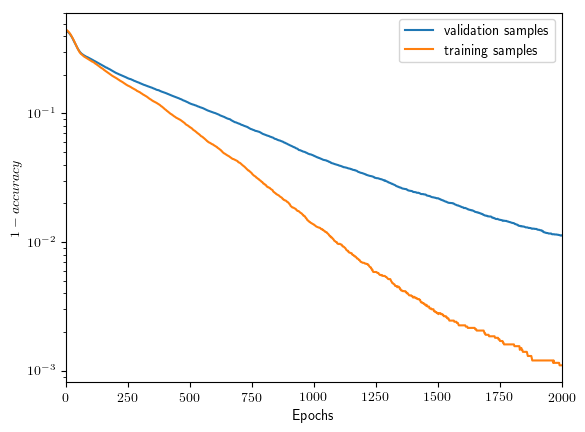
\includegraphics[width=\textwidth]{accuracy-20k.png}
 \captionof{figure}{Accuracy on the training and the validation sets for the 2D Ising model classification samples using the neural network trained for $2000$ epochs on $20\,000$ samples. Note that neither training or validation sampels in this plot represent the critical samples around the Curie temperature.\label{fig:nn_accuracy_20k}}
\end{figure}

With more data available, the model performs better. Increasing the training data set size to the entirety of the Mehta data (still retaining all critical samples for validation only), we retrain the network and arrive at the very satisfactory validation accuracy of $99.97\%$ (non-critical). Please note that this means we are missclassifying only a total of $22$ configurations, out of the $65\,000$ total. On the critical samples, the fully trained model performs marginally better, correctly classifying an additional $293$ states for a total critical accuracy of $95.47\%$. 



\section{Conclusion}
\lipsum[11]

\onecolumn{
\printbibliography
}

\end{document}



